\documentclass[11pt]{article}

\usepackage[margin=1in]{geometry}
\usepackage{amsmath,amssymb}
\usepackage{array}
\usepackage{booktabs}
\usepackage{graphicx}
\usepackage{caption}
\usepackage{hyperref}
\setlength{\emergencystretch}{3em}

\hypersetup{
  colorlinks=true,
  linkcolor=blue,
  citecolor=blue,
  urlcolor=blue
}

\title{Sample Alignment and Cohort Shift as Determinants\\of Cancer Multi-Omics Prediction Reliability:\\A Benchmark and Stress-Test Study}
\author{
Zhequan Hu\textsuperscript{1},
Xingang Bi\textsuperscript{1,*}\\
\textsuperscript{1}Department of Urology, National Cancer Center, Beijing, China\\
Cancer Hospital, Chinese Academy of Medical Sciences\\
and Peking Union Medical College, Beijing, China\\
\textsuperscript{*}Corresponding author: Professor Xingang Bi, bixingang@csco.org.cn
}
\date{\today}

\begin{document}
\maketitle

\begin{abstract}
\textbf{Background:} Cancer multi-omics prediction studies often emphasize model scores, but their reliability also depends on whether omics layers are aligned to the same tumor sample, whether modalities have comparable coverage, and whether external cohorts match the source cohort. We designed a data-centric benchmark with a predefined analysis hierarchy: five TCGA cancer-internal tasks as the primary benchmark, simulated sample-mismatch stress tests, a seven-model 10-fold model-family benchmark, an exploratory 10-cancer endpoint landscape screen, and a BRCA external-validation case study.

\textbf{Results:} The primary tasks covered UCEC molecular subtype, COADREAD molecular subtype, HNSC HPV status, KIRC grade, and PRAD pathologic T stage. At the cBioPortal sample-identifier level, all five task tables contained one unique labelled tumor-sample row per patient, no duplicate sample identifiers, and at least 98.8\% complete core-modality coverage. Simulated mismatch of non-mRNA omics rows reduced macro F1 in a task- and model-dependent manner, including drops in both tree-based and neural fusion comparators. In the seven-model 10-fold benchmark, the leading model family varied by task; exploratory fold-level effect sizes did not support a universal architecture winner. The exploratory endpoint screen identified 21 candidate within-cancer tasks across the 10 TCGA cohorts, but these were used only to map task availability and apparent difficulty. In the BRCA case study, CPTAC 2020 was more separable from the TCGA/METABRIC source distribution than SCAN-B or SMC in the marker-expression space, and external macro F1 varied by cohort and model.

\textbf{Conclusions:} Within these public benchmark settings, sample alignment, modality coverage, endpoint biology, and cohort shift were major determinants of multi-omics prediction reliability. Future cancer multi-omics benchmarks should report alignment audits and mismatch stress tests alongside model scores.
\end{abstract}

\noindent\textbf{Keywords:} multi-omics; sample alignment; domain shift; cancer prediction; TCGA; external validation; benchmark

\section{Introduction}

Cancer multi-omics studies integrate complementary molecular layers such as transcriptomics, copy-number alteration, methylation, protein abundance, and mutation profiles. These data can reveal subtype structure and tumor biology that is not visible from a single assay \cite{tcga_brca_2012,hoadley_pancancer_2018}. As machine learning methods for multi-omics prediction have become increasingly complex, benchmarking has often focused on model architecture and aggregate performance \cite{wang_mogonet_2021,leng_benchmark_2022}. However, high model scores alone do not establish that a multi-omics workflow is reliable.

Three data-level issues are especially important. First, multi-omics fusion assumes that the molecular vectors being fused belong to the same biological sample. If expression from one sample is accidentally paired with copy-number, methylation, or mutation features from another sample, the marginal distribution of each modality can remain plausible while the cross-modal biological relationship is broken. Second, not all modalities have comparable sample and feature coverage. In public cancer resources, protein measurements are often sparser than transcriptomic or mutation features, and naive early fusion can turn a nominally multi-omics table into a heavily imputed table. Third, external validation cohorts can differ from the source cohort because of assay platforms, processing pipelines, enrollment criteria, and label distributions. This cohort shift can alter model behavior even when the prediction label is nominally the same.

These issues are well recognized in high-throughput biology through work on batch effects and dataset shift \cite{johnson_combat_2007,leek_batch_2010,quionero_dataset_shift_2009}, but they are not always quantified in predictive multi-omics benchmarking. The present manuscript intentionally changes the question from whether a particular architecture wins to how much data alignment, modality coverage, and cohort shift shape the reliability of multi-omics prediction.

The primary benchmark in this study is a five-task TCGA cancer-internal analysis with explicit sample-alignment and modality-coverage audits. Around that primary benchmark, we add three secondary analyses: a controlled mismatch stress test, a seven-model 10-fold model-family comparison, and a BRCA external-validation case study using source-to-external cohort-shift summaries. We also include an exploratory 10-cancer endpoint landscape screen to show that clinically interpretable within-cancer tasks are available beyond the five deeply analysed tasks. This hierarchy is intentional: the manuscript does not claim that one model architecture is universally best, nor that external validation has been completed for all cancer types. Instead, it asks how alignment, coverage, endpoint biology, and cohort shift should be made visible when cancer multi-omics prediction models are benchmarked.

\section{Data}

\subsection{TCGA cancer-internal tasks}

We used five TCGA PanCancer Atlas cancer-internal prediction tasks assembled from cBioPortal-accessible molecular and clinical data \cite{cerami_cbioportal_2012,gao_cbioportal_2013,hoadley_pancancer_2018}. Each task was defined within a single cancer type, so the model predicted a clinically or biologically meaningful endpoint rather than cancer type itself. The tasks were UCEC molecular subtype, COADREAD molecular subtype, HNSC HPV status, KIRC histologic grade, and PRAD pathologic T stage \cite{tcga_ucec_2013,tcga_coadread_2012,tcga_hnsc_2015,tcga_kirc_2013,tcga_prad_2015}. Table~\ref{tab:tasks} summarizes the task definitions.

\begin{table}[ht]
\centering
\caption{Cancer-internal tasks used for the alignment and mismatch benchmark.}
\resizebox{\textwidth}{!}{%
\begin{tabular}{lllr}
\toprule
Task & Cancer type & Prediction target & Labelled samples \\
\midrule
UCEC molecular subtype & UCEC & CN-high, CN-low, MSI, POLE & 507 \\
COADREAD molecular subtype & COADREAD & CIN, MSI, genome-stable & 449 \\
HNSC HPV status & HNSC & HPV-positive versus HPV-negative & 487 \\
KIRC grade & KIRC & G1/G2 versus G3/G4 & 504 \\
PRAD pathologic T stage & PRAD & T2 versus T3/T4 & 487 \\
\bottomrule
\end{tabular}
}
\label{tab:tasks}
\end{table}

The available molecular feature blocks were mRNA expression, GISTIC copy-number alteration, log2 copy-number alteration, methylation, RPPA protein abundance, and mutation. The mismatch stress test used a core multi-omics feature set consisting of mRNA, GISTIC copy-number alteration, methylation, and mutation. RPPA was excluded from the core stress test because its feature-level observed fraction was low across the five tasks.

\subsection{Ten-cancer PanCancer audit}

To strengthen the multi-cancer reliability analysis, we also audited the full 10-cancer TCGA PanCancer table used in the broader project. This table contained 5957 primary tumor samples from BRCA, COADREAD, GBM, HNSC, KIRC, LUAD, LUSC, OV, PRAD, and UCEC. The same IMPACT468-based molecular feature blocks were available: mRNA expression, GISTIC copy-number alteration, log2 copy-number alteration, methylation, RPPA, and mutation. This audit was not used to claim clinical utility of cancer-type classification; instead, it served to show how strongly cancer identity structures the molecular feature space and how modality coverage differs across cancer types.

We further used the same 10-cancer TCGA PanCancer clinical records to discover additional within-cancer endpoint candidates. The search covered clinically interpretable labels that could be harmonized across at least one cancer type, including low- versus high-grade disease, molecular or histologic subtype, early- versus advanced-stage disease, and low- versus high-pathologic T stage. These expanded endpoints were used only as an exploratory task landscape and difficulty screen; the five curated cancer-internal tasks remained the deeply analysed alignment, mismatch, and model-family benchmark.

\subsection{BRCA external-validation case study}

For the cohort-shift component, we used a BRCA marker-panel case study rather than a pan-cancer external-validation analysis. TCGA-BRCA and METABRIC formed the source training/validation pool, and three external BRCA cohorts were evaluated: CPTAC 2020, SMC 2018, and GSE96058/SCAN-B \cite{tcga_brca_2012,curtis_metabric_2012,pereira_metabric_2016,krug_cptac_2020,gse96058}. The common feature space for the shift analysis was an 83-gene expression marker panel. The prediction target was a five-class PAM50-like molecular subtype label: Basal, Her2, LumA, LumB, or Normal.

\subsection{Sample unit and alignment key}

All tables were represented as one row per labelled tumor sample. The primary alignment key was \texttt{sampleId}. Patient-level labels were merged to sample-level molecular rows through \texttt{patientId} only when the original clinical label was patient-level. This design ensured that all molecular blocks in a row were intended to describe the same tumor sample before any simulated mismatch was introduced.

\section{Methods}

\subsection{Study design and analysis hierarchy}

To avoid treating all analyses as equal sources of evidence, we organized the study into a primary benchmark, secondary stress tests and model comparisons, an exploratory scope screen, and one external-validation case study (Table~\ref{tab:study_design}). The five TCGA cancer-internal tasks were the only tasks used for the complete alignment, mismatch, model-family, Liquid/CfC, noise, and medical-interpretation workflow.

\begin{table}[ht]
\centering
\caption{Study design and interpretation hierarchy.}
\label{tab:study_design}
\begingroup
\footnotesize
\setlength{\tabcolsep}{3pt}
\begin{tabular}{>{\raggedright\arraybackslash}p{0.16\textwidth}>{\raggedright\arraybackslash}p{0.20\textwidth}>{\raggedright\arraybackslash}p{0.31\textwidth}>{\raggedright\arraybackslash}p{0.23\textwidth}}
\toprule
Analysis tier & Data & Main purpose & Interpretation role \\
\midrule
Primary benchmark & Five TCGA cancer-internal tasks & Audit sample alignment and modality coverage & Main evidence base \\
Stress test & Same five tasks & Simulate broken multi-omics sample pairing & Robustness and failure-mode analysis \\
Model-family benchmark & Same five tasks & Compare seven classical and neural model families under 10-fold CV & Architecture comparison; effect-size oriented \\
Exploratory scope screen & 10 TCGA PanCancer cohorts & Discover 21 candidate within-cancer clinical endpoints & Task landscape and difficulty screen only \\
External case study & BRCA source and external cohorts & Quantify source-to-external cohort shift in an 83-gene marker space & BRCA-specific domain-shift example \\
\bottomrule
\end{tabular}
\endgroup
\end{table}

\subsection{Modality coverage audit}

For each cancer-internal task and modality, we counted the number of molecular features, the number of labelled rows with at least one observed feature, and the feature-level missing fraction. This audit was used to distinguish broadly observed core modalities from sparse modalities. Missing values were handled by training-split median imputation in all predictive models.

\subsection{Sample-level alignment audit}

Because the central stress test depends on whether the original multi-omics rows are sample-aligned, we performed an explicit cBioPortal-level sample audit before introducing any simulated mismatch. For each cancer-internal task, we counted labelled rows, unique \texttt{sampleId} values, duplicate sample rows, unique \texttt{patientId} values, patients with more than one labelled sample, primary solid tumor rows, and the fraction of rows with at least one observed feature in every core modality. Clinical labels stored at patient level were merged to molecular rows only through the corresponding \texttt{patientId}; because no patient contributed more than one labelled sample in the audited task tables, this merge did not create repeated patient-level labels across multiple tumor samples. The mismatch-core modality set was mRNA, GISTIC copy number, methylation, and mutation. The expanded-core modality set additionally included log2 copy number. This audit tests whether the modelling table is one row per labelled tumor sample and whether core molecular blocks are present at the sample level. It does not prove aliquot-level molecular provenance across portion, analyte, and aliquot barcodes; that distinction is treated as a limitation of using harmonized public cBioPortal tables.

\subsection{Simulated sample-mismatch stress test}

Let \(x_i^{(m)}\) denote modality \(m\) for sample \(i\). In an aligned multi-omics table, the row
\[
X_i = \{x_i^{(\mathrm{mRNA})}, x_i^{(\mathrm{CNA})}, x_i^{(\mathrm{methylation})}, x_i^{(\mathrm{mutation})}\}
\]
contains molecular features from the same tumor sample. To simulate sample-level multi-omics mismatch, we selected a fraction \(\rho \in \{0, 0.10, 0.25, 0.50, 0.75, 1.00\}\) of rows and independently permuted the non-mRNA modalities across those rows:
\[
\tilde{X}_i(\rho)=\{x_i^{(\mathrm{mRNA})}, x_{\pi_{\mathrm{CNA}}(i)}^{(\mathrm{CNA})}, x_{\pi_{\mathrm{meth}}(i)}^{(\mathrm{methylation})}, x_{\pi_{\mathrm{mut}}(i)}^{(\mathrm{mutation})}\}.
\]
This stress test preserves the marginal distribution of each modality but breaks the biological pairing between modalities for the affected rows. We evaluated two scenarios: mismatch introduced in the training set only, and mismatch introduced in the test set only.

Each task was split into 70\% training and 30\% test sets using stratified sampling. Splitting was repeated with seeds 42, 43, and 44. We evaluated two practical baseline models: class-balanced logistic regression and ExtraTrees. The single-modality mRNA model served as a reference anchor. Macro F1 was the primary metric, with balanced accuracy and ROC-AUC reported as secondary metrics.

To connect the Liquid/CfC applicability analysis with the alignment stress test, we repeated the mismatch experiment for Liquid/CfC and small-Liquid/CfC using the same mismatch rates and seeds. The 70\% training portion was internally split into training and validation subsets for neural early stopping. For training-mismatch experiments, non-mRNA modalities were permuted in the neural training subset while the validation and test sets remained aligned. For test-mismatch experiments, the neural model was trained on aligned data and evaluated on the mismatched test set.

\subsection{Liquid/CfC model implementation}

The Liquid/CfC models were implemented as modality-sequence neural fusion modules, not as temporal clinical models. Each omics block was first transformed by a modality-specific encoder consisting of a linear projection, ReLU activation, dropout, and layer normalization. A learned modality embedding was then added. The resulting sequence \(z_1,\ldots,z_T\) represented omics modalities in a fixed order. For the seven-model 10-fold benchmark, the order was mRNA, GISTIC copy number, log2 copy number, methylation, and mutation. For the mismatch stress test, the order was mRNA, GISTIC copy number, methylation, and mutation to match the perturbation core. We used this sequence only as a structured fusion device: the order lets the model update a shared state as each modality is observed, but it should not be interpreted as biological time.

For a modality embedding \(z_t\) and hidden state \(h_{t-1}\), the implemented CfC-style update was
\[
r_t=\mathrm{softplus}\left(W_r[z_t,h_{t-1}]+b_r\right)+10^{-3},
\]
\[
\alpha_t=1-\exp(-r_t\Delta t), \quad \Delta t=1,
\]
\[
c_t=\tanh(W_x z_t+W_h h_{t-1}), \quad
g_t=\sigma(W_g[z_t,h_{t-1}]+b_g),
\]
\[
q_t=g_t\odot c_t+(1-g_t)\odot h_{t-1},
\]
\[
h_t=(1-\alpha_t)\odot h_{t-1}+\alpha_t\odot q_t,
\]
with \(h_0=0\). The final hidden state was passed through layer normalization and a linear classifier. The full Liquid/CfC model used an embedding dimension of 64 and hidden dimension of 96. The small-Liquid/CfC model used an embedding dimension of 32 and hidden dimension of 48, reducing trainable parameters from 192,866--193,060 to 84,914--85,012 across the five tasks, or approximately 44\% of the full model size.

Neural models were trained with class-weighted cross-entropy, AdamW, learning rate \(10^{-3}\), weight decay \(10^{-4}\), batch size 64, and gradient clipping at norm 5.0. In the 10-fold model-family benchmark, neural models used a maximum of 60 epochs and early-stopping patience of 8 epochs. In the Liquid/CfC mismatch stress test, the maximum was 35 epochs with patience 5. Early stopping used validation macro one-vs-rest ROC-AUC when defined and validation balanced accuracy otherwise.

\subsection{Expanded baseline benchmark and statistical comparison}

To address model-family baseline performance independently of the simulated mismatch experiment, we also performed 10-fold stratified cross-validation on the same five TCGA cancer-internal tasks using seven model families: elastic-net logistic regression, Random Forest, ExtraTrees, HistGradientBoosting, early-fusion multilayer perceptron (MLP), modality-sequence Liquid/CfC, and small-Liquid/CfC. The core aligned modalities were mRNA, GISTIC copy number, log2 copy number, methylation, and mutation; RPPA was excluded from this expanded benchmark because the coverage audit showed sparse RPPA observations.

For each fold, preprocessing parameters were fitted only on the training portion. Neural models used an internal validation subset for early stopping. Macro F1 was the primary endpoint, and one-vs-rest macro ROC-AUC was reported as a secondary endpoint. For each task, we identified the highest mean macro F1 model and summarized its fold-level difference from the runner-up. We reported the mean paired fold-level F1 difference, bootstrap 95\% confidence intervals for that mean difference, and an exploratory Wilcoxon signed-rank test with an exact sign-test fallback when required. Because cross-validation folds are not independent biological samples, these \(p\) values were interpreted only as exploratory paired fold-level diagnostics, not as definitive population-level inferential tests. Holm-adjusted values were provided to avoid overemphasizing isolated fold-level contrasts. Finally, Gaussian noise was added to standardized test features to estimate a robustness elbow for the best model in each task.

\subsection{BRCA domain-shift quantification}

For the BRCA external-validation case study, we quantified source-to-external cohort shift in the common 83-gene expression marker space. The source domain was the TCGA-BRCA/METABRIC training split. For each external cohort, we computed two shift summaries.

First, we fitted a logistic domain classifier to distinguish source samples from external samples using cross-validation. Because the sign of the domain classifier score is arbitrary, we report domain separability as
\[
A_{\mathrm{sep}}=\max(AUC, 1-AUC),
\]
so values near 0.5 indicate little separability and values closer to 1 indicate stronger cohort separability. Second, after median imputation and standardization fitted on the source domain, we computed the mean absolute difference between source and external feature means:
\[
D_{\mathrm{mean}} = \frac{1}{p}\sum_{j=1}^{p}\left|\bar{z}_{j,\mathrm{external}}-\bar{z}_{j,\mathrm{source}}\right|.
\]
We then trained logistic regression and ExtraTrees subtype classifiers on the source training split and evaluated them on the source validation split and the three external cohorts.

\subsection{Ten-cancer PanCancer extension}

For the 10-cancer PanCancer extension, we computed modality coverage by cancer type and assay. We also quantified how easily each cancer type could be separated from the remaining nine cancer types using mRNA features alone. For each cancer type \(c\), we fitted a one-vs-rest logistic classifier and reported cross-validated ROC-AUC:
\[
A_c = \mathrm{AUC}\left(\hat{p}(y=c), \mathbb{1}\{y=c\}\right).
\]
Finally, we compared the best macro F1 from the 10-class PanCancer cancer-type task with the best macro F1 values from the five within-cancer endpoint tasks. This comparison was intended to distinguish between-cancer tissue identity signals from the more difficult clinical or molecular endpoint prediction tasks within a cancer type.

\subsection{Exploratory clinical endpoint discovery}

To avoid limiting the scope analysis to the five curated tasks, we systematically queried TCGA PanCancer clinical attributes for BRCA, COADREAD, GBM, HNSC, KIRC, LUAD, LUSC, OV, PRAD, and UCEC. Candidate endpoints were retained when they could be mapped to a clinically interpretable classification target and each retained class had at least 40 labelled samples. Stage was harmonized as early versus advanced disease, pathologic T stage as low versus high local extension, histologic grade as low versus high grade, and subtype labels as cancer-specific molecular or histologic subtype classes.

For a lightweight difficulty estimate, each candidate endpoint was evaluated with three-fold stratified cross-validation using two baselines: elastic-net logistic regression and ExtraTrees. Missing values were median-imputed inside each training fold. To reduce dimensionality and keep the expanded screen comparable across cancers, the top 300 features were selected within each training fold using univariate ANOVA \(F\)-statistics before model fitting. Macro F1 was the primary screening metric. Because endpoints were discovered and screened within the same public resource, this analysis is subject to selection bias and was interpreted only as an exploratory task-availability and apparent-difficulty landscape, not as validated evidence for the 21 endpoints.

\subsection{Medical interpretation mapping}

For each cancer-internal endpoint, we summarized the clinical or biological target, the expected dominant biology, why multi-omics information may be relevant, and how the observed model pattern should be interpreted medically. This table was not used as a statistical test; it was included to make the benchmark clinically interpretable and to distinguish biologically plausible model behavior from leaderboard-style model ranking.

\section{Results}

\subsection{Sample-level alignment audit supports the core modelling table}

The alignment audit verified that each of the five cancer-internal modelling tables contained one labelled row per unique tumor sample, with no duplicate \texttt{sampleId} values and no patients contributing multiple labelled samples (Table~\ref{tab:alignment_audit}). All rows were primary solid tumor samples. The mismatch-core modalities were fully present at the sample level in UCEC, COADREAD, and HNSC, and nearly complete in KIRC (98.8\%) and PRAD (98.8\%). This audit establishes the aligned baseline from which simulated mismatch was introduced; the mismatch experiment therefore tests sensitivity to broken sample pairing rather than correcting a known duplicate-key problem in the original tables.

\begin{table}[ht]
\centering
\caption{Sample-level alignment audit for the five cancer-internal tasks. Core completeness refers to rows with at least one observed feature in mRNA, GISTIC copy number, methylation, and mutation. RPPA is shown as sample-level presence of any RPPA feature and is distinct from feature-level sparsity.}
\resizebox{\textwidth}{!}{%
\begin{tabular}{lrrrrrr}
\toprule
Task & Labelled rows & Unique samples & Duplicate samples & Unique patients & Multi-sample patients & Core-complete rows \\
\midrule
UCEC molecular subtype & 507 & 507 & 0 & 507 & 0 & 507 (100.0\%) \\
COADREAD molecular subtype & 449 & 449 & 0 & 449 & 0 & 449 (100.0\%) \\
HNSC HPV status & 487 & 487 & 0 & 487 & 0 & 487 (100.0\%) \\
KIRC grade & 504 & 504 & 0 & 504 & 0 & 498 (98.8\%) \\
PRAD pathologic T stage & 487 & 487 & 0 & 487 & 0 & 481 (98.8\%) \\
\bottomrule
\end{tabular}
}
\label{tab:alignment_audit}
\end{table}

\subsection{Modality coverage differs strongly across omics layers}

Core mRNA, copy-number, methylation, and mutation features had high observed fractions across the five TCGA cancer-internal tasks. In contrast, RPPA was sparse, with feature-level observed fractions ranging from 5.7\% in HNSC HPV status to 12.4\% in KIRC grade (Figure~\ref{fig:coverage}). This result supports treating modality coverage as a pre-modeling audit step rather than assuming that all nominally available omics layers should be fused.

\begin{figure}[ht]
\centering
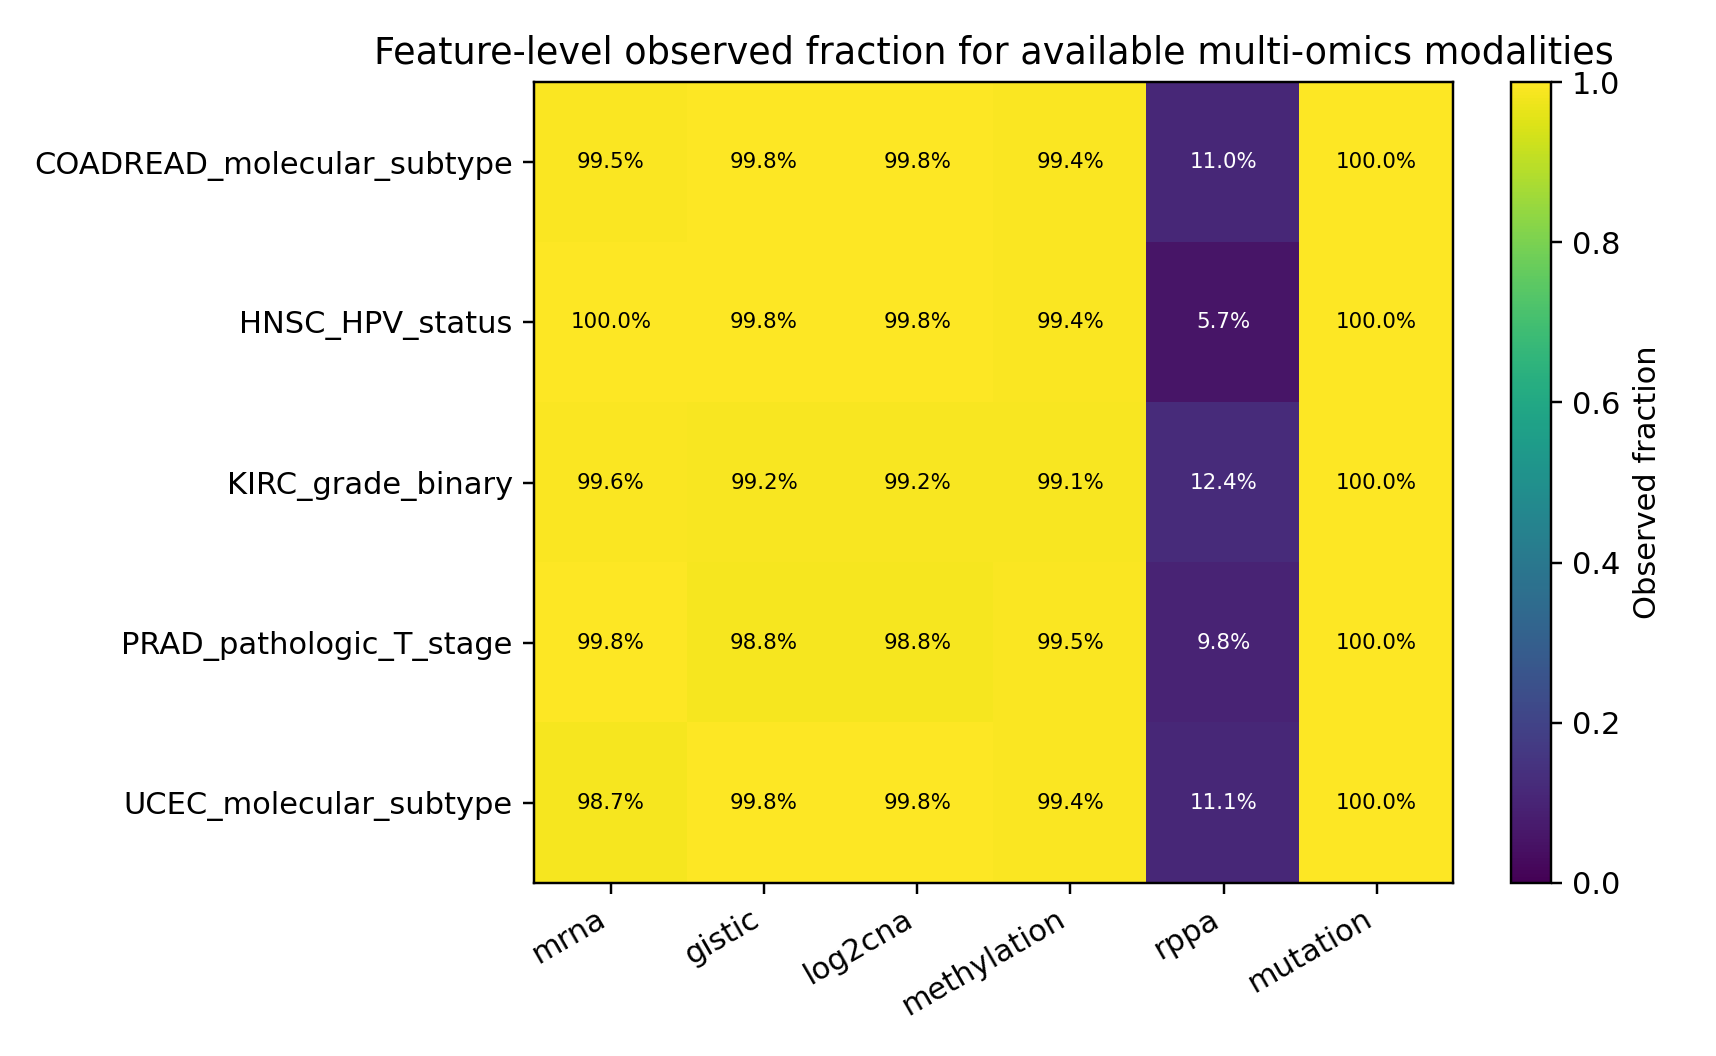
\includegraphics[width=\textwidth]{figures/modality_coverage_heatmap.png}
\caption{Feature-level observed fraction across available multi-omics modalities in five TCGA cancer-internal tasks. RPPA coverage was substantially lower than mRNA, copy-number, methylation, and mutation coverage.}
\label{fig:coverage}
\end{figure}

\subsection{The 10-cancer audit reveals broad assay heterogeneity}

At the full PanCancer level, mutation, copy-number, and methylation features had high observed fractions in most cancers, but coverage was not uniform across assays or cancer types. GBM had low observed mRNA feature coverage in the processed table (26\%), OV showed intermediate mRNA coverage (51\%), and RPPA remained sparse across all 10 cancer types (approximately 5\%--12\% observed feature fraction; Figure~\ref{fig:pancancer_coverage}). This broader audit confirms that modality coverage is not merely a task-specific concern: it is a recurring property of public multi-omics resources.

\begin{figure}[ht]
\centering
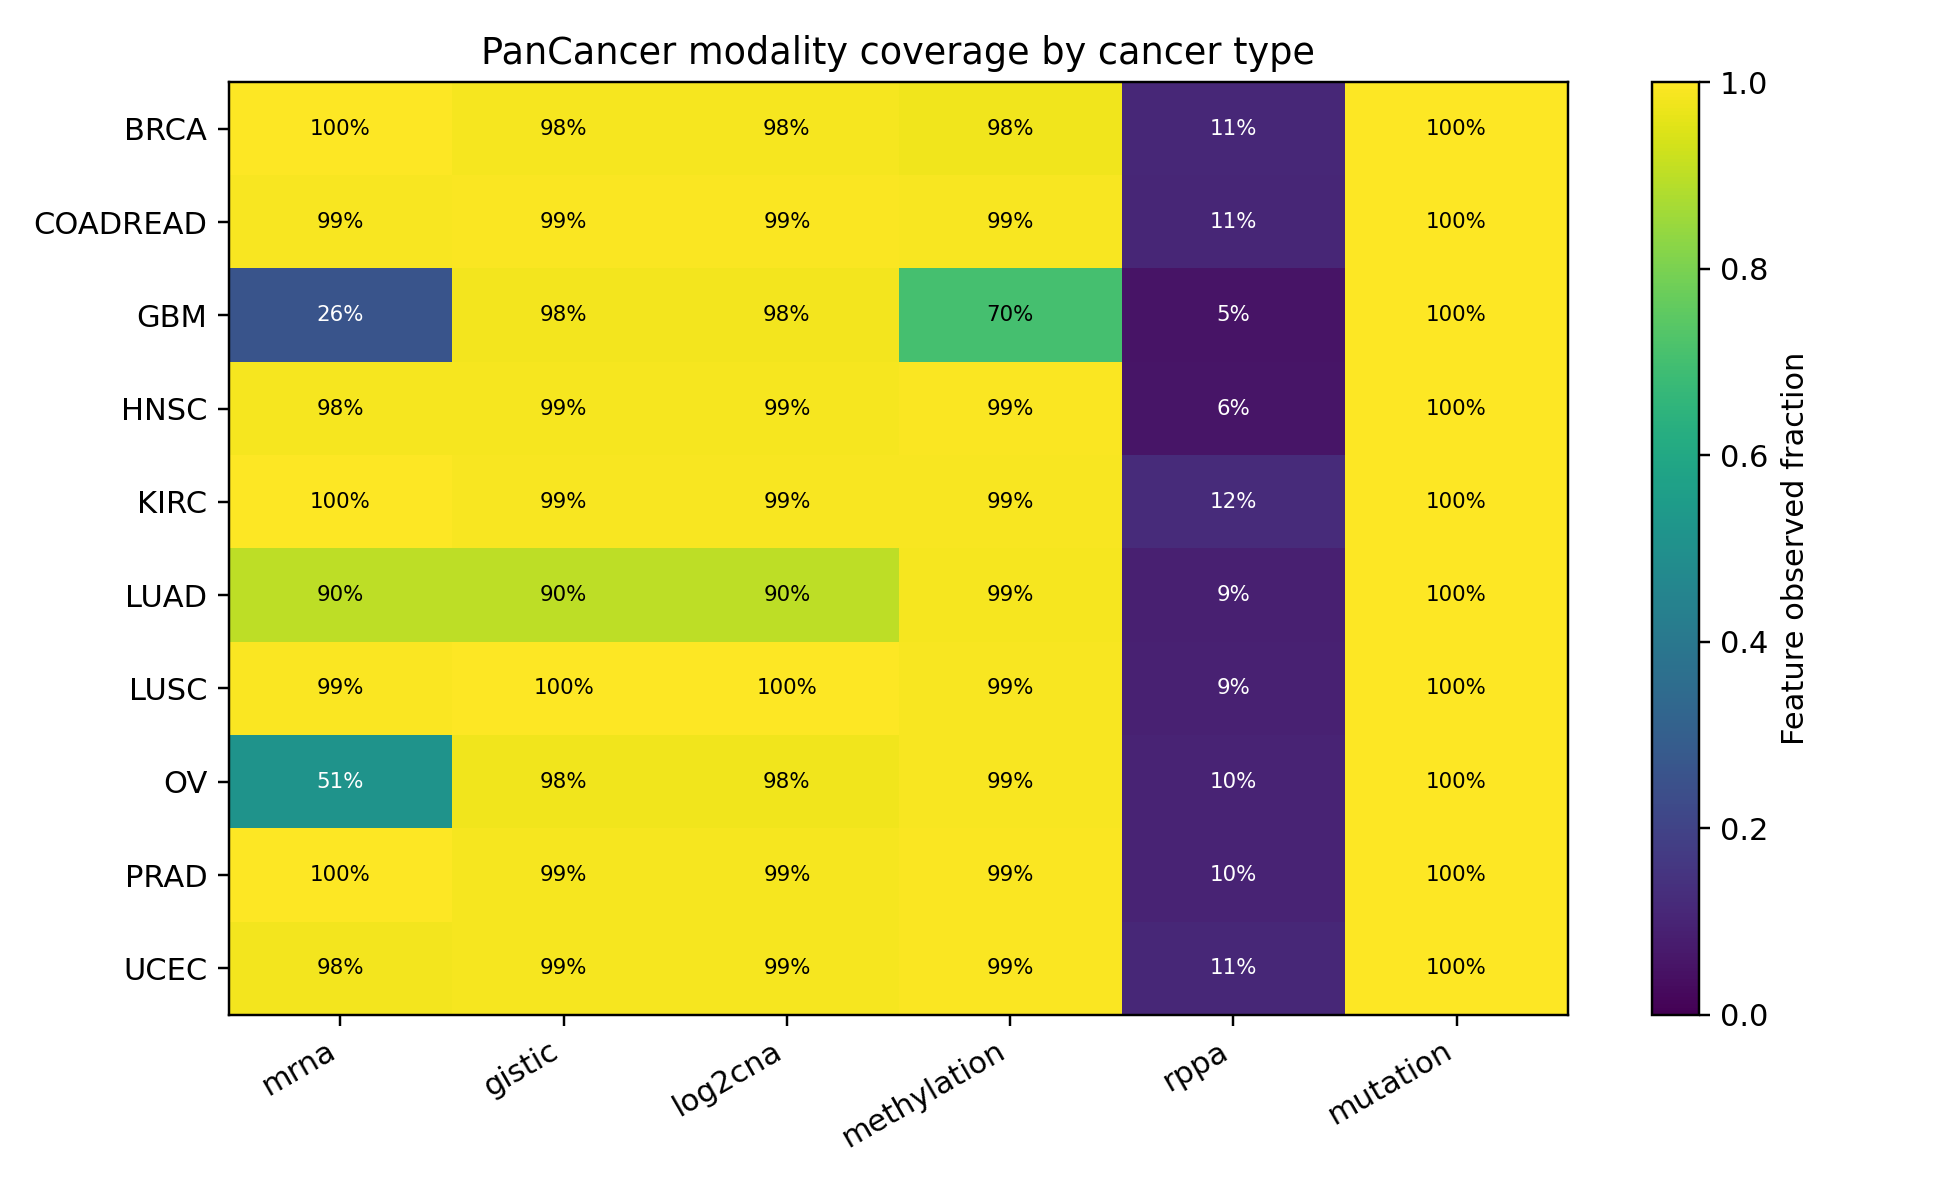
\includegraphics[width=\textwidth]{figures/pancancer_modality_coverage_by_cancer.png}
\caption{PanCancer modality coverage by cancer type. Values show the feature-level observed fraction for each assay block in the 10-cancer TCGA PanCancer table. RPPA was consistently sparse, and some cancers also showed reduced mRNA coverage in the processed feature table.}
\label{fig:pancancer_coverage}
\end{figure}

\subsection{Exploratory endpoint discovery broadens the task landscape}

Across the 10 TCGA PanCancer cohorts, the exploratory clinical endpoint screen identified 21 candidate within-cancer tasks with sufficient class support (Figure~\ref{fig:expanded_scope_availability}). These included four grade tasks, four molecular or histologic subtype tasks, six early- versus advanced-stage tasks, and seven pathologic T-stage tasks. The available task count differed by cancer type: BRCA, COADREAD, HNSC, KIRC, UCEC, LUAD, LUSC, OV, and PRAD each contributed at least one clinically interpretable endpoint, whereas GBM did not meet the predefined endpoint and class-count criteria in this screen.

\begin{figure}[ht]
\centering
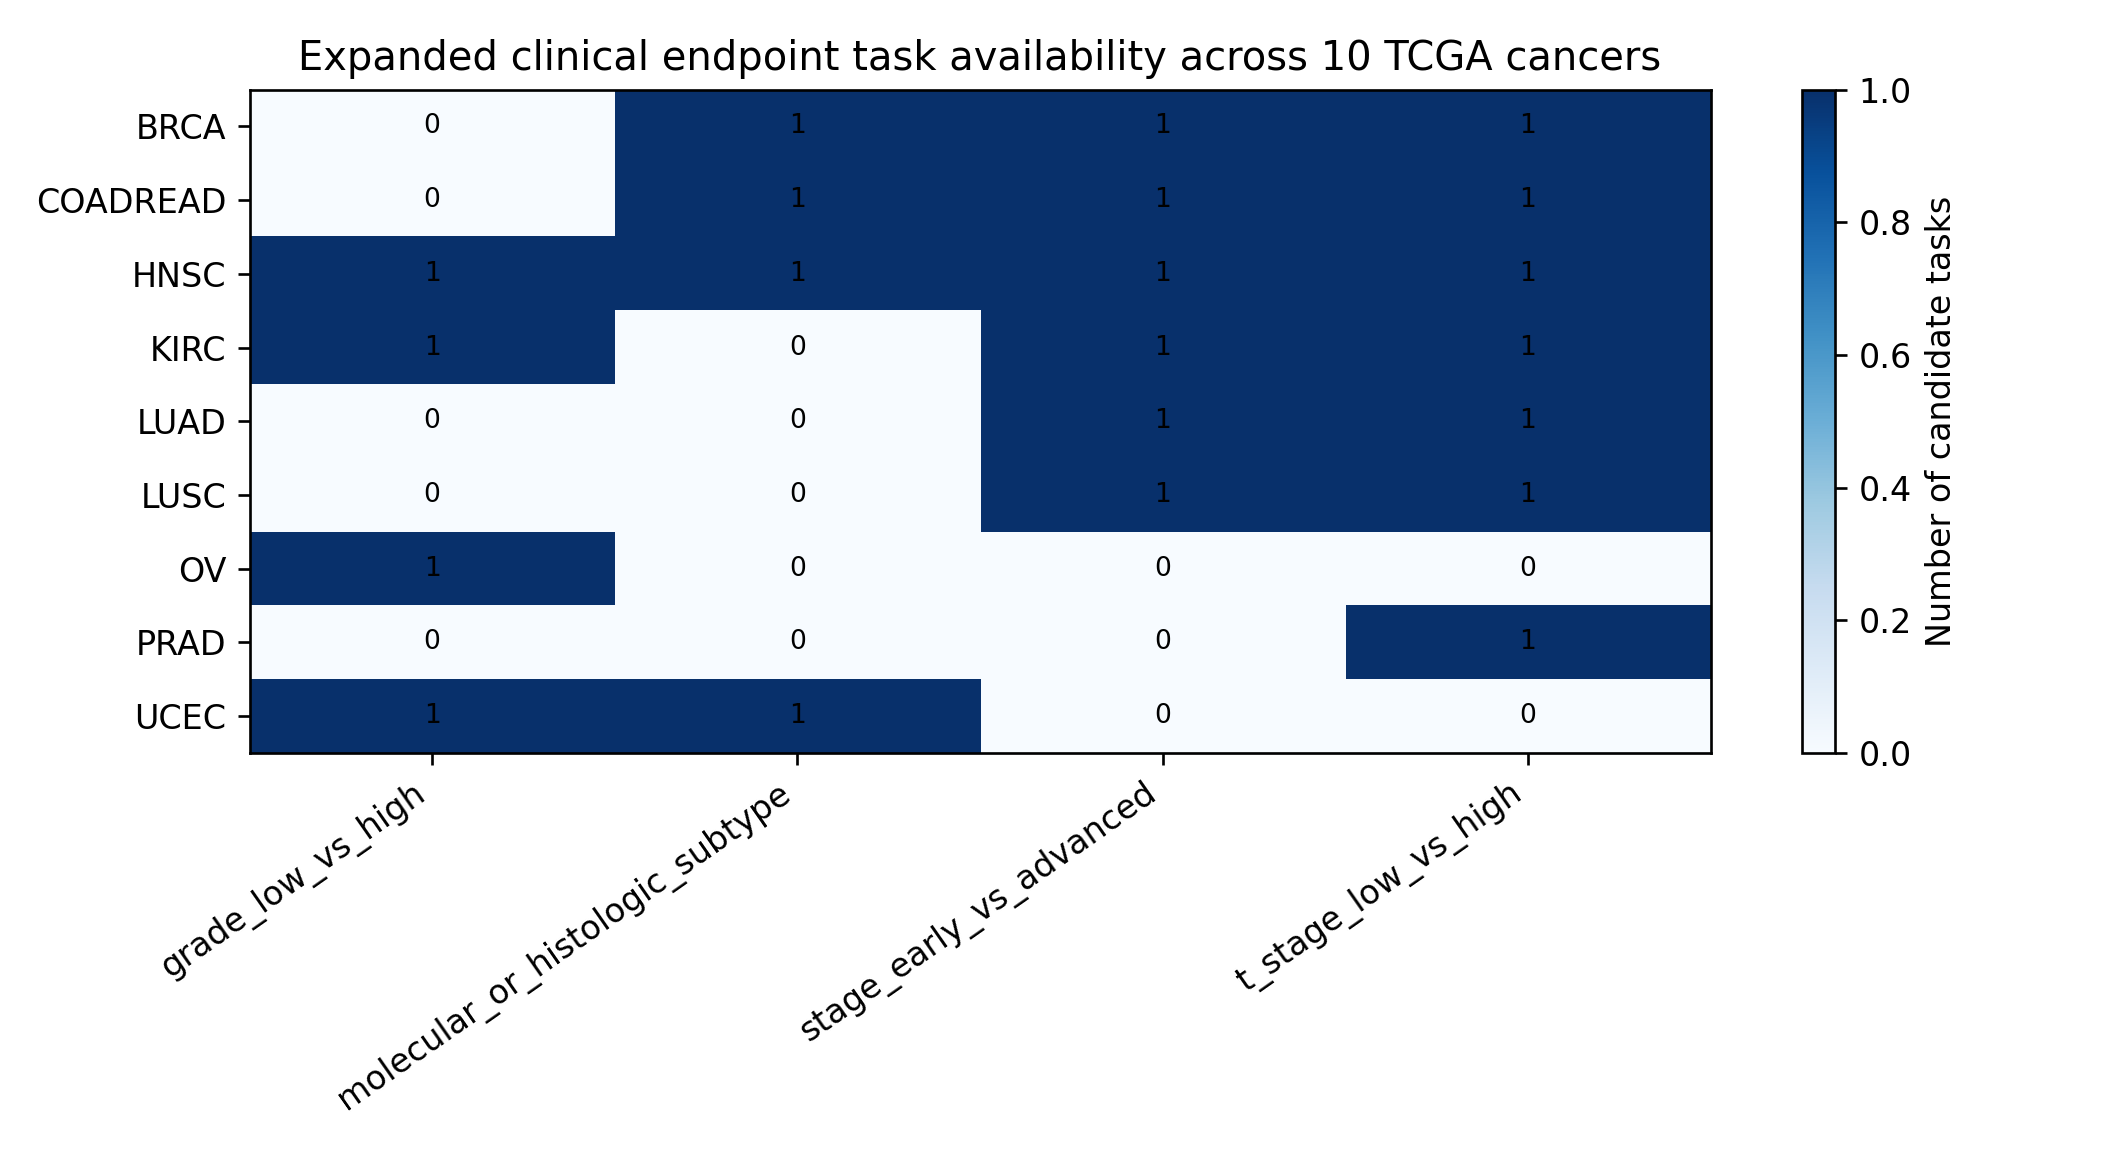
\includegraphics[width=0.90\textwidth]{figures/expanded_scope_task_availability.png}
\caption{Expanded within-cancer endpoint availability across the 10 TCGA PanCancer cohorts. Candidate tasks were retained only when labels could be harmonized into a clinically interpretable endpoint and each retained class had at least 40 labelled samples.}
\label{fig:expanded_scope_availability}
\end{figure}

The lightweight three-fold baseline screen showed substantial variation in endpoint difficulty (Figure~\ref{fig:expanded_scope_f1}; Table~\ref{tab:expanded_scope}). Molecular or histologic subtype tasks were the most learnable group, with best-task macro F1 values ranging from 0.8178 to 0.9387. Grade prediction was heterogeneous, ranging from 0.5582 in OV to 0.8341 in UCEC. Stage and pathologic T-stage tasks were generally harder, with best-task macro F1 ranges of 0.5152--0.6893 and 0.5050--0.7049, respectively. These results expand the benchmark from a small set of hand-curated endpoints to a broader map of candidate task availability and difficulty while preserving the main manuscript's focus on alignment, mismatch sensitivity, and cohort shift.

\begin{figure}[ht]
\centering
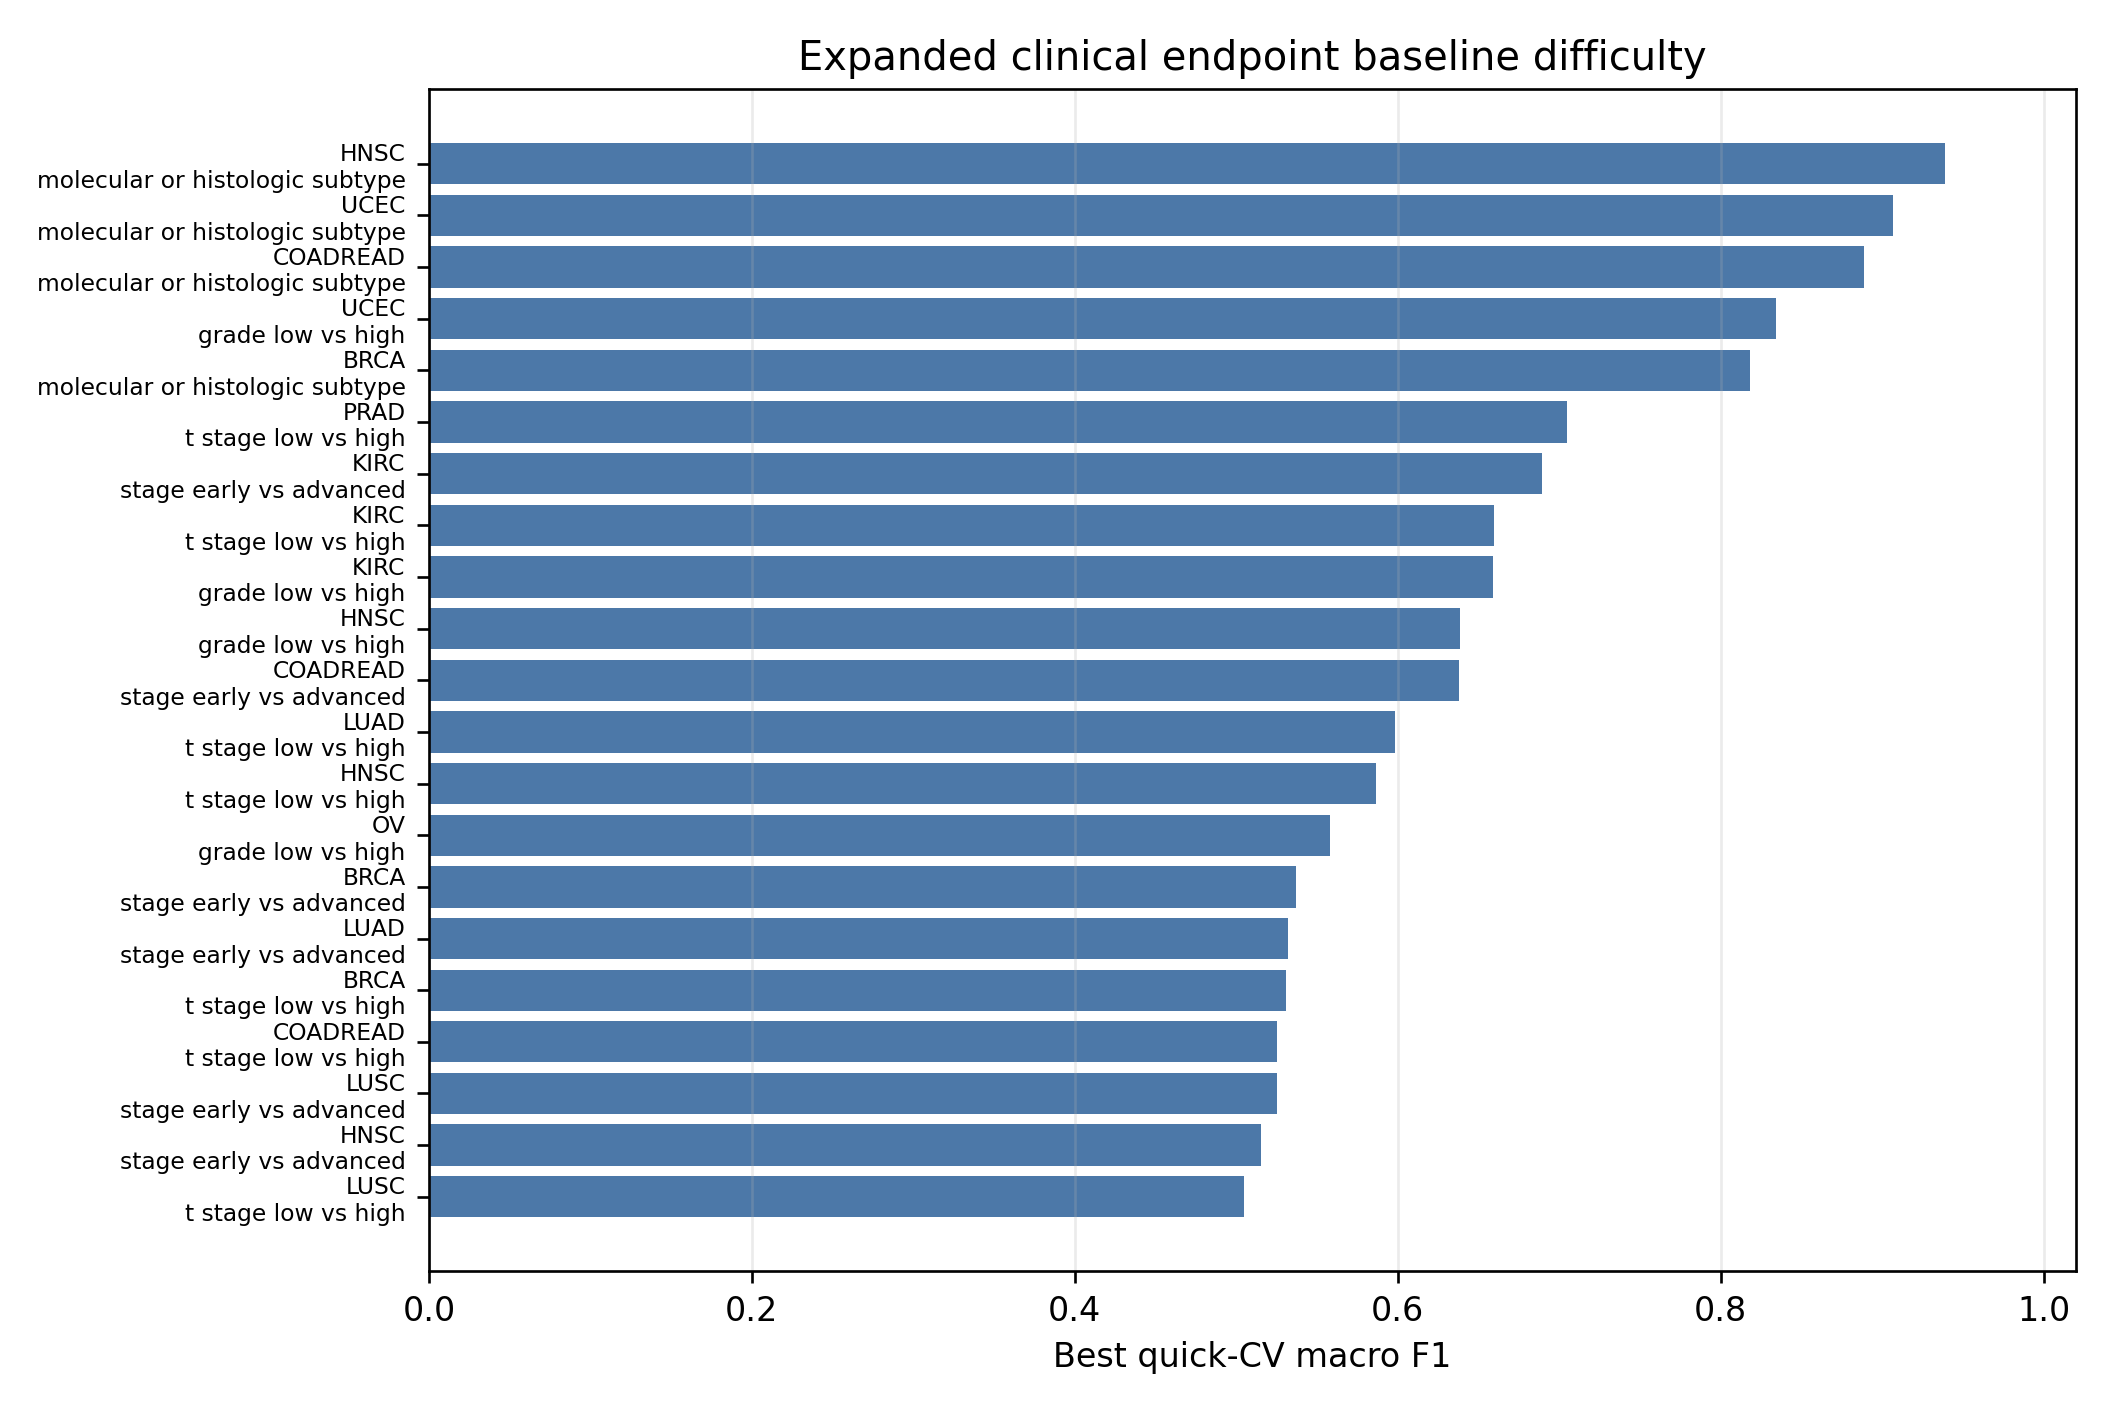
\includegraphics[width=\textwidth]{figures/expanded_scope_endpoint_f1.png}
\caption{Quick baseline difficulty screen for expanded within-cancer endpoints. Values show the better macro F1 of elastic-net logistic regression and ExtraTrees under three-fold cross-validation with training-fold feature selection.}
\label{fig:expanded_scope_f1}
\end{figure}

\begin{table}[ht]
\centering
\caption{Expanded endpoint families discovered across the 10-cancer TCGA PanCancer clinical screen. Macro F1 ranges use the better of elastic-net logistic regression and ExtraTrees for each task in the lightweight three-fold screen.}
\label{tab:expanded_scope}
\resizebox{\textwidth}{!}{%
\begin{tabular}{lrrrl}
\toprule
Endpoint family & Candidate tasks & Cancers represented & Best macro F1 range & Highest-scoring task \\
\midrule
Grade low vs high & 4 & 4 & 0.5582--0.8341 & UCEC grade \\
Molecular or histologic subtype & 4 & 4 & 0.8178--0.9387 & HNSC subtype \\
Stage early vs advanced & 6 & 6 & 0.5152--0.6893 & KIRC stage \\
Pathologic T stage low vs high & 7 & 7 & 0.5050--0.7049 & PRAD pathologic T stage \\
\bottomrule
\end{tabular}
}
\end{table}

\subsection{Simulated sample mismatch reduces multi-omics prediction performance}

When non-mRNA omics layers were permuted across samples, multi-omics performance declined in a task- and model-dependent manner (Figure~\ref{fig:mismatch}). The largest aligned-to-fully-misaligned macro F1 drops occurred for COADREAD molecular subtype using ExtraTrees (0.8893 to 0.5008; drop 0.3885) and UCEC molecular subtype using ExtraTrees (0.9141 to 0.5914; drop 0.3227). Logistic regression was less sensitive in COADREAD but still showed a notable UCEC drop (0.9088 to 0.6943; drop 0.2145). KIRC grade and PRAD pathologic T stage showed smaller drops, suggesting that some tasks were driven mainly by mRNA or by robust single-modality signals.

\begin{figure}[ht]
\centering
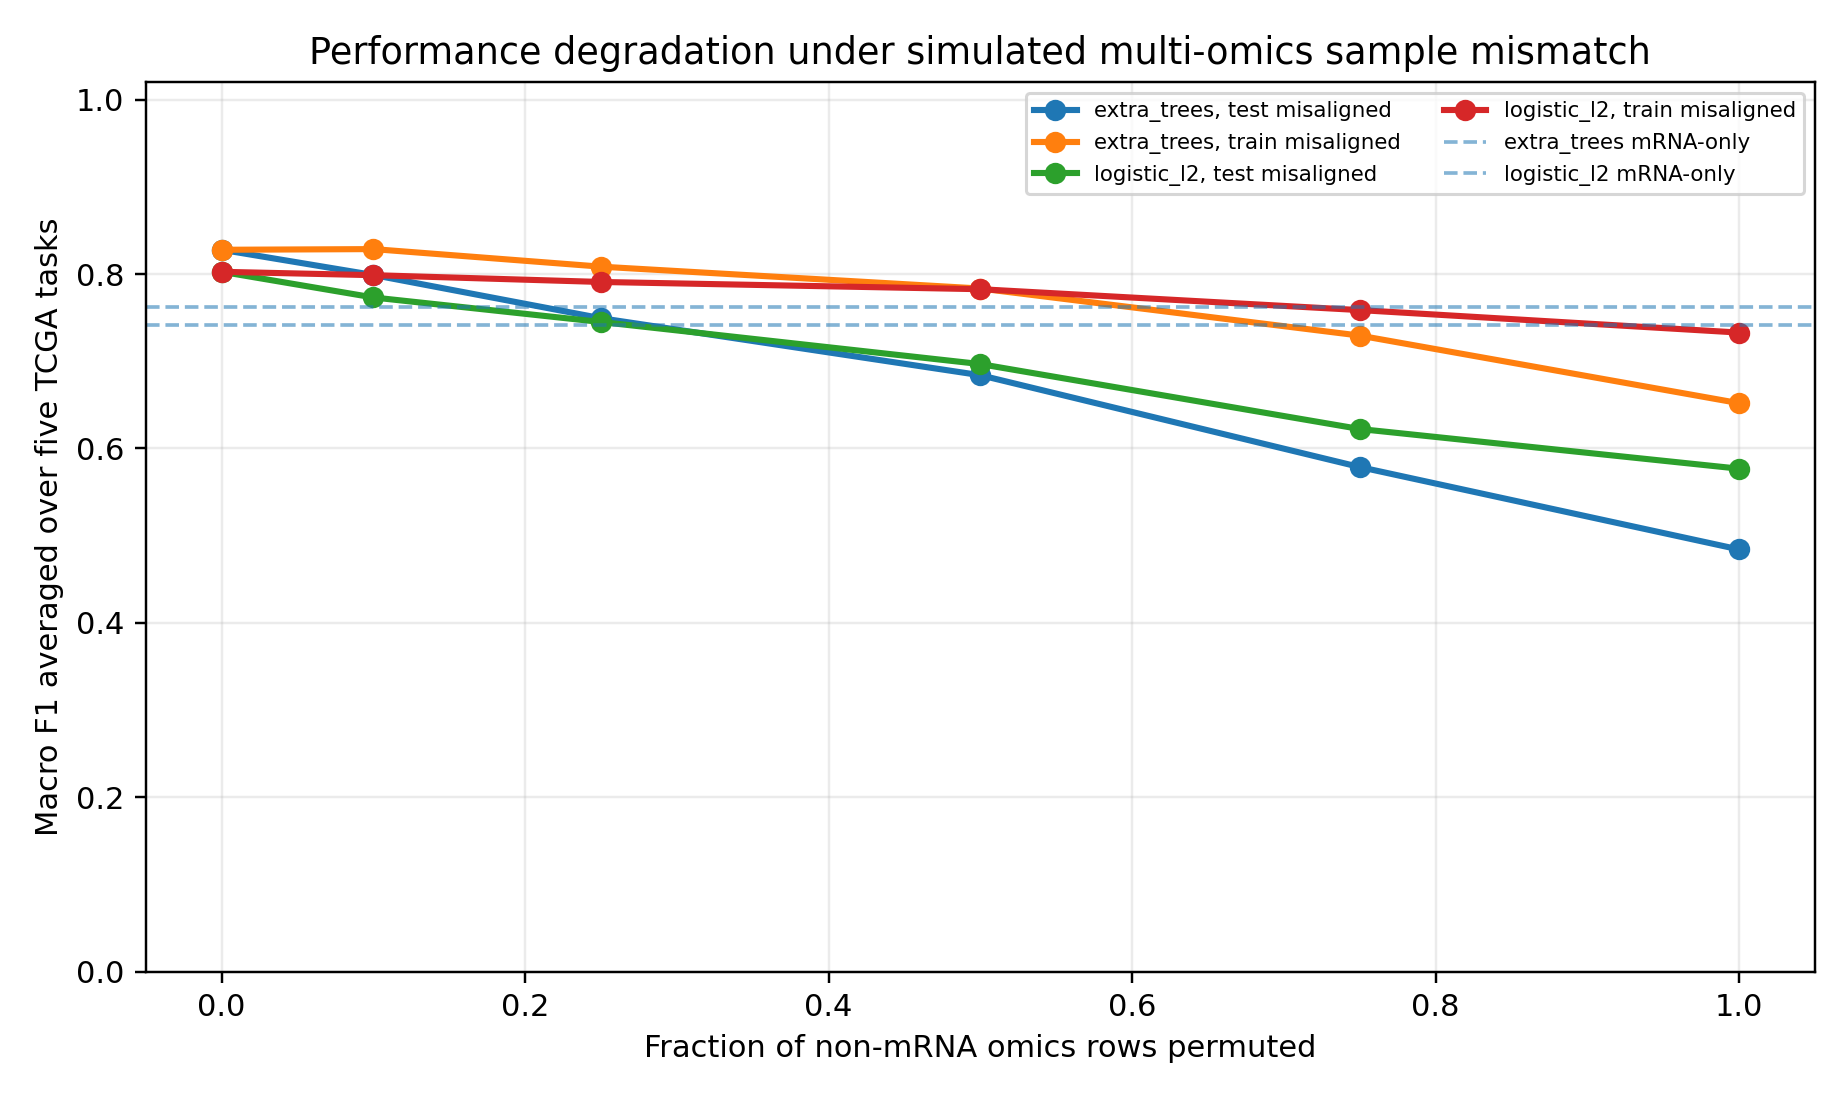
\includegraphics[width=\textwidth]{figures/misalignment_degradation.png}
\caption{Macro F1 degradation under simulated sample mismatch. Non-mRNA omics rows were permuted at increasing rates while preserving each modality's marginal distribution. Lines summarize mean macro F1 across the five TCGA cancer-internal tasks and three random seeds. Dashed lines indicate mRNA-only reference performance.}
\label{fig:mismatch}
\end{figure}

\begin{table}[ht]
\centering
\caption{Aligned versus fully misaligned training data in the cancer-internal stress test.}
\resizebox{\textwidth}{!}{%
\begin{tabular}{llrrr}
\toprule
Task & Model & Aligned macro F1 & Fully misaligned macro F1 & Drop \\
\midrule
COADREAD molecular subtype & ExtraTrees & 0.8893 & 0.5008 & 0.3885 \\
UCEC molecular subtype & ExtraTrees & 0.9141 & 0.5914 & 0.3227 \\
UCEC molecular subtype & Logistic L2 & 0.9088 & 0.6943 & 0.2145 \\
HNSC HPV status & ExtraTrees & 0.9573 & 0.8405 & 0.1168 \\
HNSC HPV status & Logistic L2 & 0.9640 & 0.9201 & 0.0439 \\
COADREAD molecular subtype & Logistic L2 & 0.8686 & 0.8323 & 0.0363 \\
KIRC grade & ExtraTrees & 0.7200 & 0.6868 & 0.0332 \\
KIRC grade & Logistic L2 & 0.6498 & 0.6206 & 0.0292 \\
PRAD pathologic T stage & Logistic L2 & 0.6215 & 0.5970 & 0.0245 \\
PRAD pathologic T stage & ExtraTrees & 0.6583 & 0.6400 & 0.0183 \\
\bottomrule
\end{tabular}
}
\label{tab:mismatch}
\end{table}

The Liquid-family mismatch extension showed the same qualitative pattern: Liquid/CfC and small-Liquid/CfC were not immune to sample-level pairing errors (Figure~\ref{fig:liquid_mismatch}). Under fully mismatched training data, the largest Liquid-family macro F1 drops occurred for COADREAD small-Liquid/CfC (0.8041 to 0.5639; drop 0.2402), UCEC Liquid/CfC (0.8982 to 0.6587; drop 0.2396), and UCEC small-Liquid/CfC (0.8487 to 0.6257; drop 0.2230). HNSC also showed drops above 0.11 for both Liquid variants, whereas KIRC and PRAD were less sensitive, particularly for full Liquid/CfC.

\begin{figure}[ht]
\centering
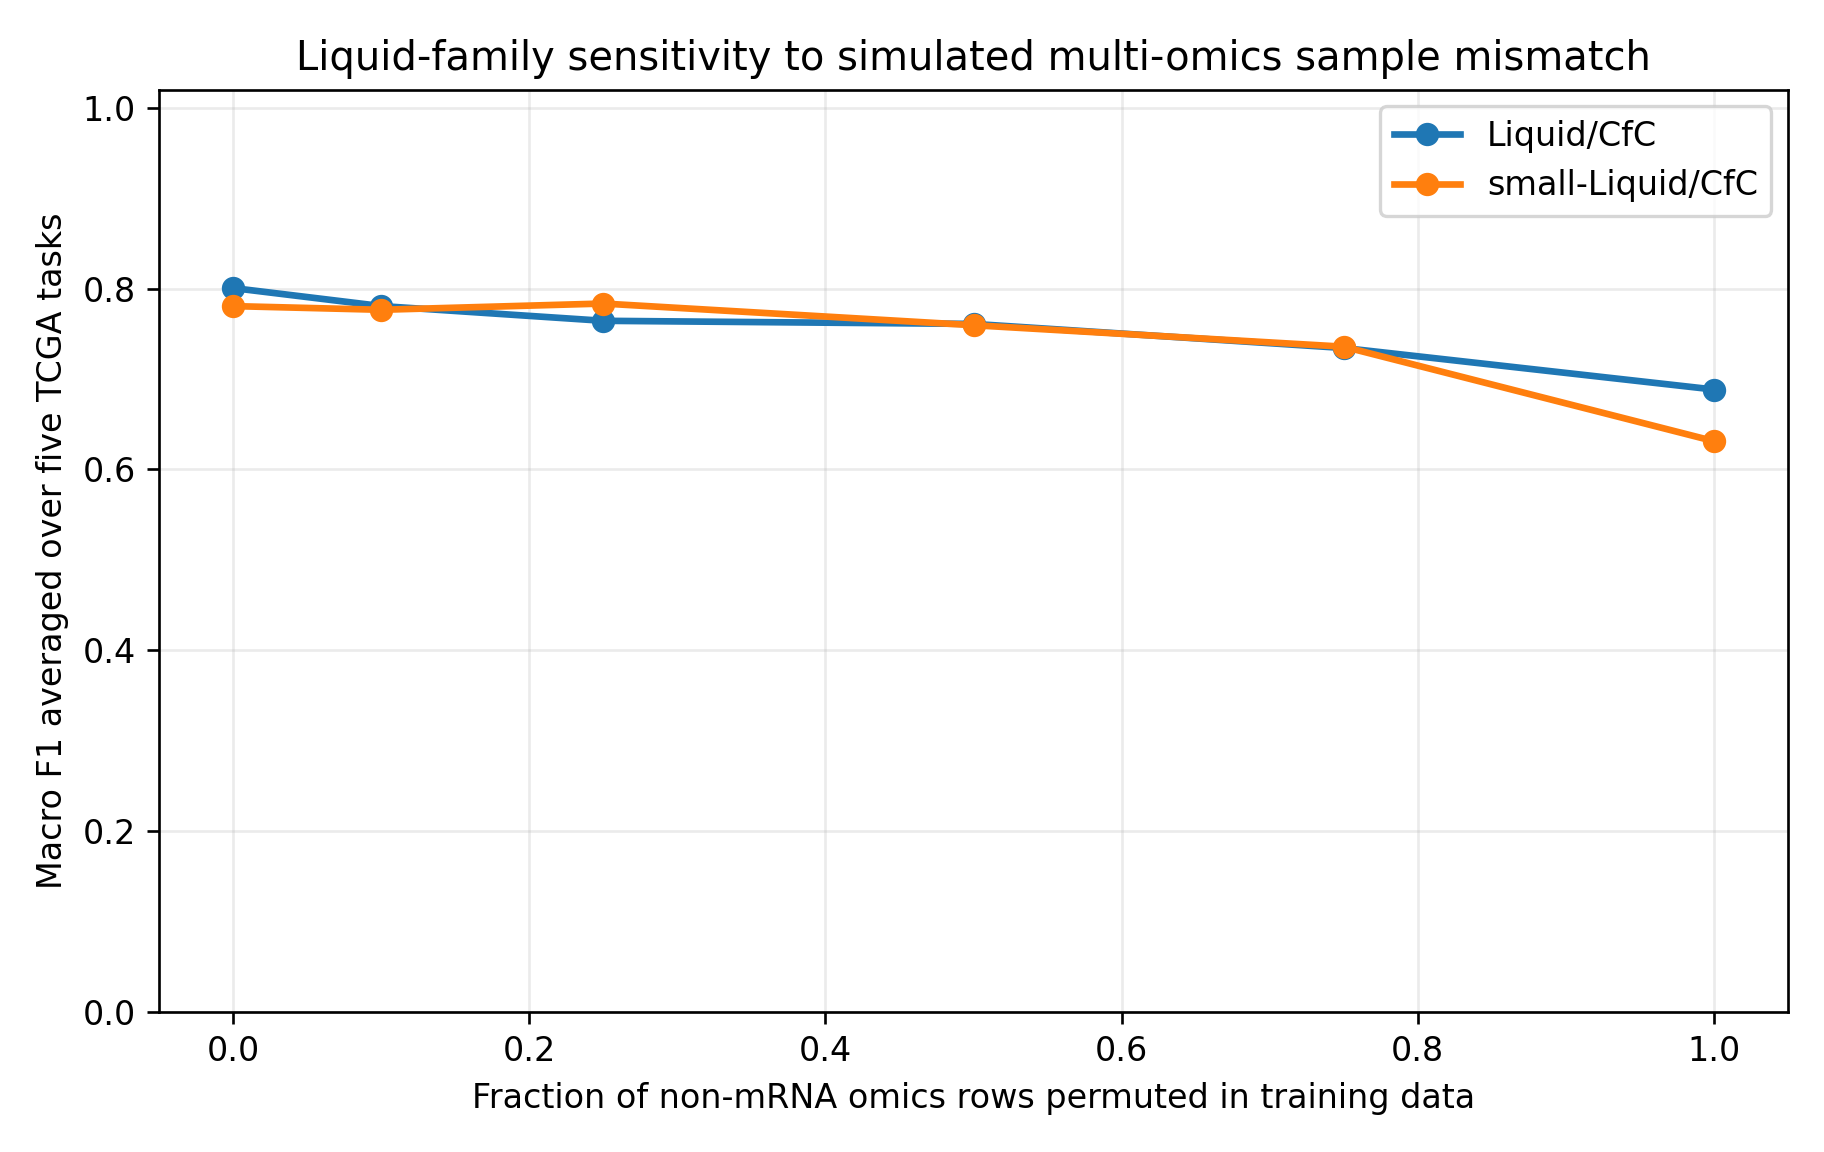
\includegraphics[width=0.86\textwidth]{figures/liquid_mismatch_degradation.png}
\caption{Liquid-family sensitivity to simulated multi-omics sample mismatch. Lines show mean macro F1 across the five TCGA cancer-internal tasks and three random seeds when non-mRNA omics rows were permuted in the training data.}
\label{fig:liquid_mismatch}
\end{figure}

\begin{table}[ht]
\centering
\caption{Liquid-family aligned versus fully misaligned training data in the cancer-internal stress test.}
\resizebox{\textwidth}{!}{%
\begin{tabular}{llrrr}
\toprule
Task & Model & Aligned macro F1 & Fully misaligned macro F1 & Drop \\
\midrule
COADREAD molecular subtype & small-Liquid/CfC & 0.8041 & 0.5639 & 0.2402 \\
UCEC molecular subtype & Liquid/CfC & 0.8982 & 0.6587 & 0.2396 \\
UCEC molecular subtype & small-Liquid/CfC & 0.8487 & 0.6257 & 0.2230 \\
COADREAD molecular subtype & Liquid/CfC & 0.8382 & 0.7010 & 0.1372 \\
HNSC HPV status & small-Liquid/CfC & 0.9236 & 0.7996 & 0.1240 \\
HNSC HPV status & Liquid/CfC & 0.9445 & 0.8259 & 0.1187 \\
PRAD pathologic T stage & small-Liquid/CfC & 0.6667 & 0.5714 & 0.0953 \\
KIRC grade & small-Liquid/CfC & 0.6601 & 0.5959 & 0.0642 \\
PRAD pathologic T stage & Liquid/CfC & 0.6690 & 0.6247 & 0.0443 \\
KIRC grade & Liquid/CfC & 0.6529 & 0.6317 & 0.0212 \\
\bottomrule
\end{tabular}
}
\label{tab:liquid_mismatch}
\end{table}

\subsection{Expanded baselines do not support a universal architecture winner}

The expanded 10-fold benchmark included seven model families across the five cancer-internal tasks (Figure~\ref{fig:expanded_baseline}). The leading model differed by task: ExtraTrees achieved the highest mean macro F1 for COADREAD molecular subtype (0.8676) and UCEC molecular subtype (0.8944), elastic-net logistic regression led HNSC HPV status (0.9469), and Random Forest led KIRC grade (0.6784) and PRAD pathologic T stage (0.6839). Liquid/CfC and small-Liquid/CfC were competitive in several tasks but were not consistently superior.

\begin{figure}[ht]
\centering
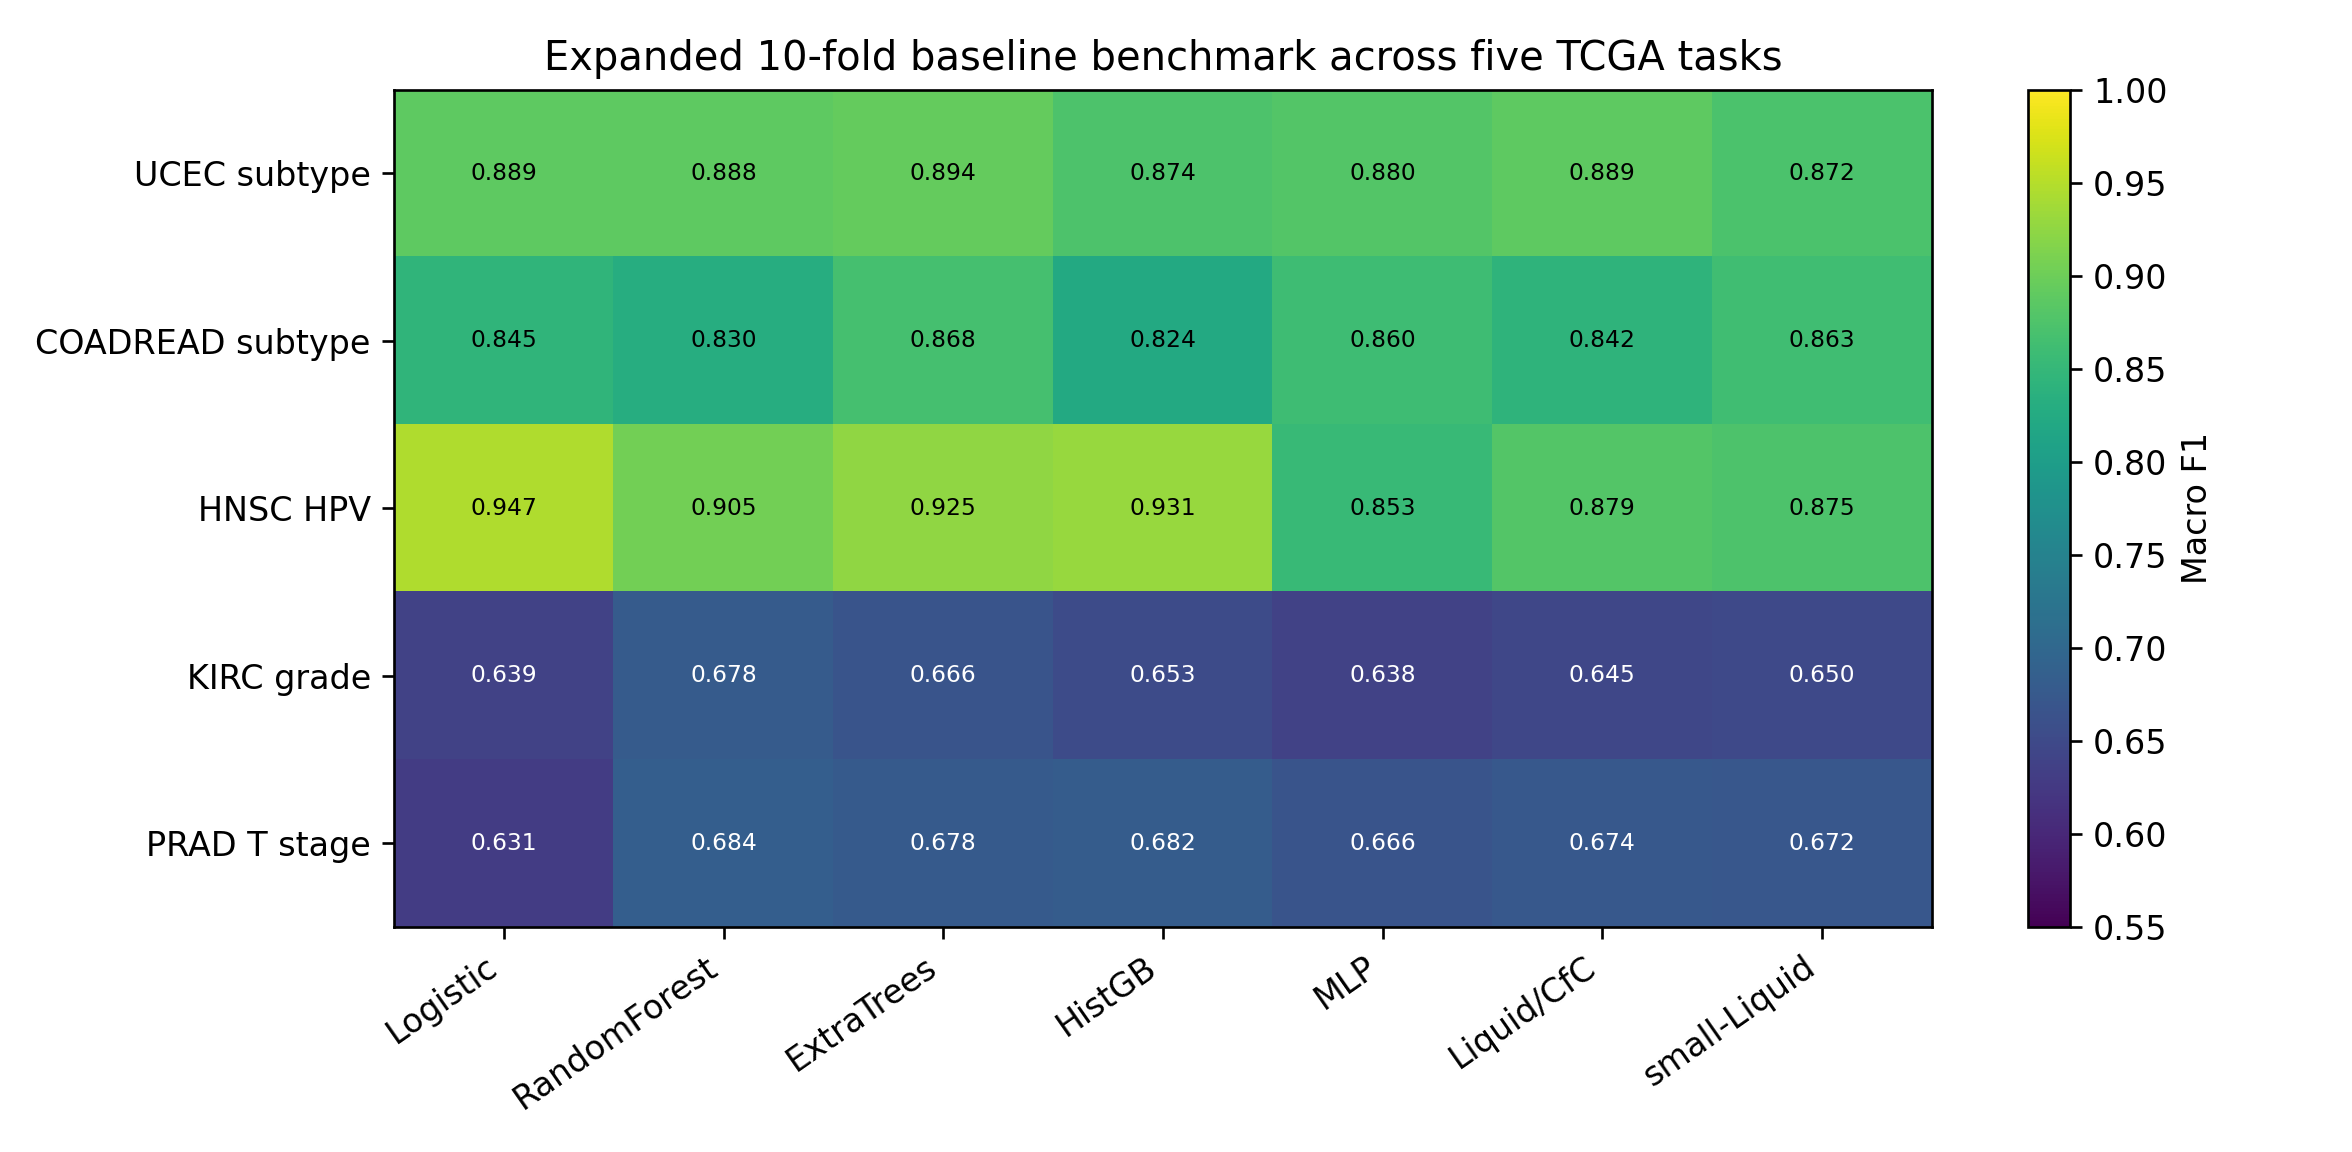
\includegraphics[width=\textwidth]{figures/expanded_baseline_cv_heatmap.png}
\caption{Expanded 10-fold baseline benchmark across five TCGA cancer-internal tasks. Values show mean macro F1 for each model family. The leading architecture differed by task, and no single model family dominated all endpoints.}
\label{fig:expanded_baseline}
\end{figure}

\begin{table}[ht]
\centering
\caption{Best 10-fold baseline model per cancer-internal task and exploratory paired top-versus-runner-up fold-level comparison.}
\resizebox{\textwidth}{!}{%
\begin{tabular}{lllrrrr}
\toprule
Task & Top model & Runner-up & Top macro F1 & Mean F1 diff & 95\% CI for diff & Exploratory Holm \(p\) \\
\midrule
COADREAD molecular subtype & ExtraTrees & small-Liquid/CfC & 0.8676 & 0.0048 & [-0.0431, 0.0514] & 1.0000 \\
HNSC HPV status & Elastic-net logistic & HistGradientBoosting & 0.9469 & 0.0159 & [-0.0141, 0.0470] & 1.0000 \\
KIRC grade & Random Forest & ExtraTrees & 0.6784 & 0.0122 & [-0.0057, 0.0310] & 1.0000 \\
PRAD pathologic T stage & Random Forest & HistGradientBoosting & 0.6839 & 0.0021 & [-0.0451, 0.0389] & 1.0000 \\
UCEC molecular subtype & ExtraTrees & Elastic-net logistic & 0.8944 & 0.0053 & [-0.0391, 0.0471] & 1.0000 \\
\bottomrule
\end{tabular}
}
\label{tab:expanded_baseline}
\end{table}

Exploratory fold-level paired comparisons reinforced the effect-size interpretation. All top-versus-runner-up confidence intervals crossed zero (Table~\ref{tab:expanded_baseline}). In the broader top-versus-all diagnostics, the clearest contrast was HNSC HPV status, where elastic-net logistic regression exceeded MLP by 0.0939 macro F1 (95\% CI 0.0444--0.1382; exploratory adjusted \(p=0.0469\)). Because CV folds are not independent biological samples, these \(p\) values were not treated as definitive inferential tests. The benchmark therefore supports a task- and data-dependent reliability interpretation rather than a claim that Liquid/CfC or any other architecture is universally best.

\subsection{Liquid/CfC serves as a task-dependent neural comparator}

The expanded benchmark also allowed us to examine where Liquid/CfC-style models were relatively strong or weak (Table~\ref{tab:liquid_applicability}). Liquid/CfC or small-Liquid/CfC was near the best model in COADREAD molecular subtype, UCEC molecular subtype, and PRAD pathologic T stage, with mean macro F1 within 0.01 of the task-leading model. However, Liquid/CfC was weaker in HNSC HPV status, where elastic-net logistic regression led by 0.0675 macro F1 over Liquid/CfC and 0.0722 over small-Liquid/CfC. In KIRC grade, Random Forest also led the Liquid variants by approximately 0.03 macro F1.

\begin{table}[ht]
\centering
\caption{Task-level interpretation of Liquid/CfC and small-Liquid/CfC performance. Delta values are relative to the best 10-fold mean macro F1 model for each task.}
\resizebox{\textwidth}{!}{%
\begin{tabular}{llrrl}
\toprule
Task & Best Liquid-family model & Rank & Delta versus best & Interpretation \\
\midrule
COADREAD molecular subtype & small-Liquid/CfC & 2 & -0.0048 & Near-best; competitive with ExtraTrees \\
UCEC molecular subtype & Liquid/CfC & 3 & -0.0059 & Near-best; no clear gap to ExtraTrees \\
PRAD pathologic T stage & Liquid/CfC & 4 & -0.0097 & Near-best, but all models were close \\
KIRC grade & small-Liquid/CfC & 4 & -0.0283 & Modestly weaker than Random Forest \\
HNSC HPV status & Liquid/CfC & 5 & -0.0675 & Weaker than elastic-net logistic regression \\
\bottomrule
\end{tabular}
}
\label{tab:liquid_applicability}
\end{table}

These findings suggest a practical boundary for using Liquid/CfC in static cancer multi-omics. Liquid-style models may be useful when the task benefits from structured cross-modality integration and when no single sparse linear signal dominates. They appear less advantageous when the endpoint is already well separated by simpler feature combinations, as in HNSC HPV status, or when tabular tree ensembles capture the relevant nonlinearities with fewer modeling assumptions, as in KIRC grade. Thus, Liquid/CfC should be treated as a comparator whose value is task-dependent rather than as a default superior architecture for cancer multi-omics tables.

\subsection{Medical interpretation links model behavior to endpoint biology}

The task-level model patterns were medically interpretable rather than arbitrary (Table~\ref{tab:medical_interpretation}). UCEC and COADREAD molecular subtypes are defined by multiple biological mechanisms, including copy-number burden, microsatellite instability, polymerase-epsilon proofreading mutations, and epigenetic or expression programs. These endpoints are plausible settings for cross-modality integration, and Liquid-family models were near-best or strongly mismatch-sensitive in both tasks. HNSC HPV status, in contrast, is a high-signal viral-oncogenesis endpoint; the strongest model was elastic-net logistic regression, suggesting that simpler expression-associated decision boundaries can be sufficient. KIRC grade and PRAD pathologic T stage are partly histopathologic or anatomic endpoints, which may explain their lower molecular predictability and the potential value of future pathology or imaging-augmented extensions.

\begin{table}[ht]
\centering
\caption{Medical interpretation of the five cancer-internal endpoints and observed model behavior.}
\begingroup
\scriptsize
\setlength{\tabcolsep}{3pt}
\begin{tabular}{>{\raggedright\arraybackslash}p{0.14\textwidth}>{\raggedright\arraybackslash}p{0.26\textwidth}>{\raggedright\arraybackslash}p{0.26\textwidth}>{\raggedright\arraybackslash}p{0.24\textwidth}}
\toprule
Task & Endpoint biology & Why multi-omics may matter & Model interpretation \\
\midrule
UCEC molecular subtype & CN-high, CN-low, MSI, and POLE subtypes reflect copy-number burden, mismatch repair deficiency, and polymerase proofreading mutations. & CNA, mutation, methylation, and expression can provide complementary subtype signals. & Liquid/CfC was near-best and mismatch-sensitive, consistent with cross-modality relevance. \\
COADREAD molecular subtype & CIN, MSI, and genome-stable colorectal cancer reflect chromosomal instability, microsatellite instability, and epigenetic/expression programs. & The endpoint combines genome instability and transcriptomic or methylation programs. & small-Liquid/CfC was near-best, although ExtraTrees had the top mean macro F1. \\
HNSC HPV status & HPV-positive disease reflects viral oncogenesis and strong transcriptional/cell-cycle signatures. & Expression signal may already separate the endpoint strongly. & Elastic-net logistic regression was strongest; Liquid/CfC was not advantageous. \\
KIRC grade & Histologic grade reflects tumor aggressiveness, hypoxia/angiogenesis, chromatin remodeling, and VHL-related biology. & Bulk molecular features may only partly capture a histopathologic phenotype. & Random Forest was strongest; pathology imaging may be a natural complementary modality. \\
PRAD pathologic T stage & T stage reflects local invasion and anatomic extension, not a purely molecular phenotype. & Molecular signal is expected to be modest and may need clinical or imaging context. & Liquid/CfC was near-best, but all models were close. \\
\bottomrule
\end{tabular}
\endgroup
\label{tab:medical_interpretation}
\end{table}

\subsection{Cancer-type classification is much easier than within-cancer endpoint prediction}

The existing PanCancer cancer-type benchmark achieved a best macro F1 of 0.9904 across 10 cancer types. In one-vs-rest analyses using mRNA features alone, every cancer type was highly separable from the remaining cancers, with AUC values ranging from 0.9721 for OV to 0.9997 for COADREAD (Figure~\ref{fig:cancer_sep}). By contrast, the five clinically or molecularly meaningful within-cancer tasks were more variable: HNSC HPV status reached 0.9505 macro F1, UCEC and COADREAD molecular subtypes were near 0.91, while PRAD pathologic T stage and KIRC grade were near 0.70 (Figure~\ref{fig:task_difficulty}). This contrast is important because a high pan-cancer cancer-type score can mostly reflect strong tissue-of-origin structure, whereas clinically useful within-cancer prediction remains harder.

\begin{figure}[ht]
\centering
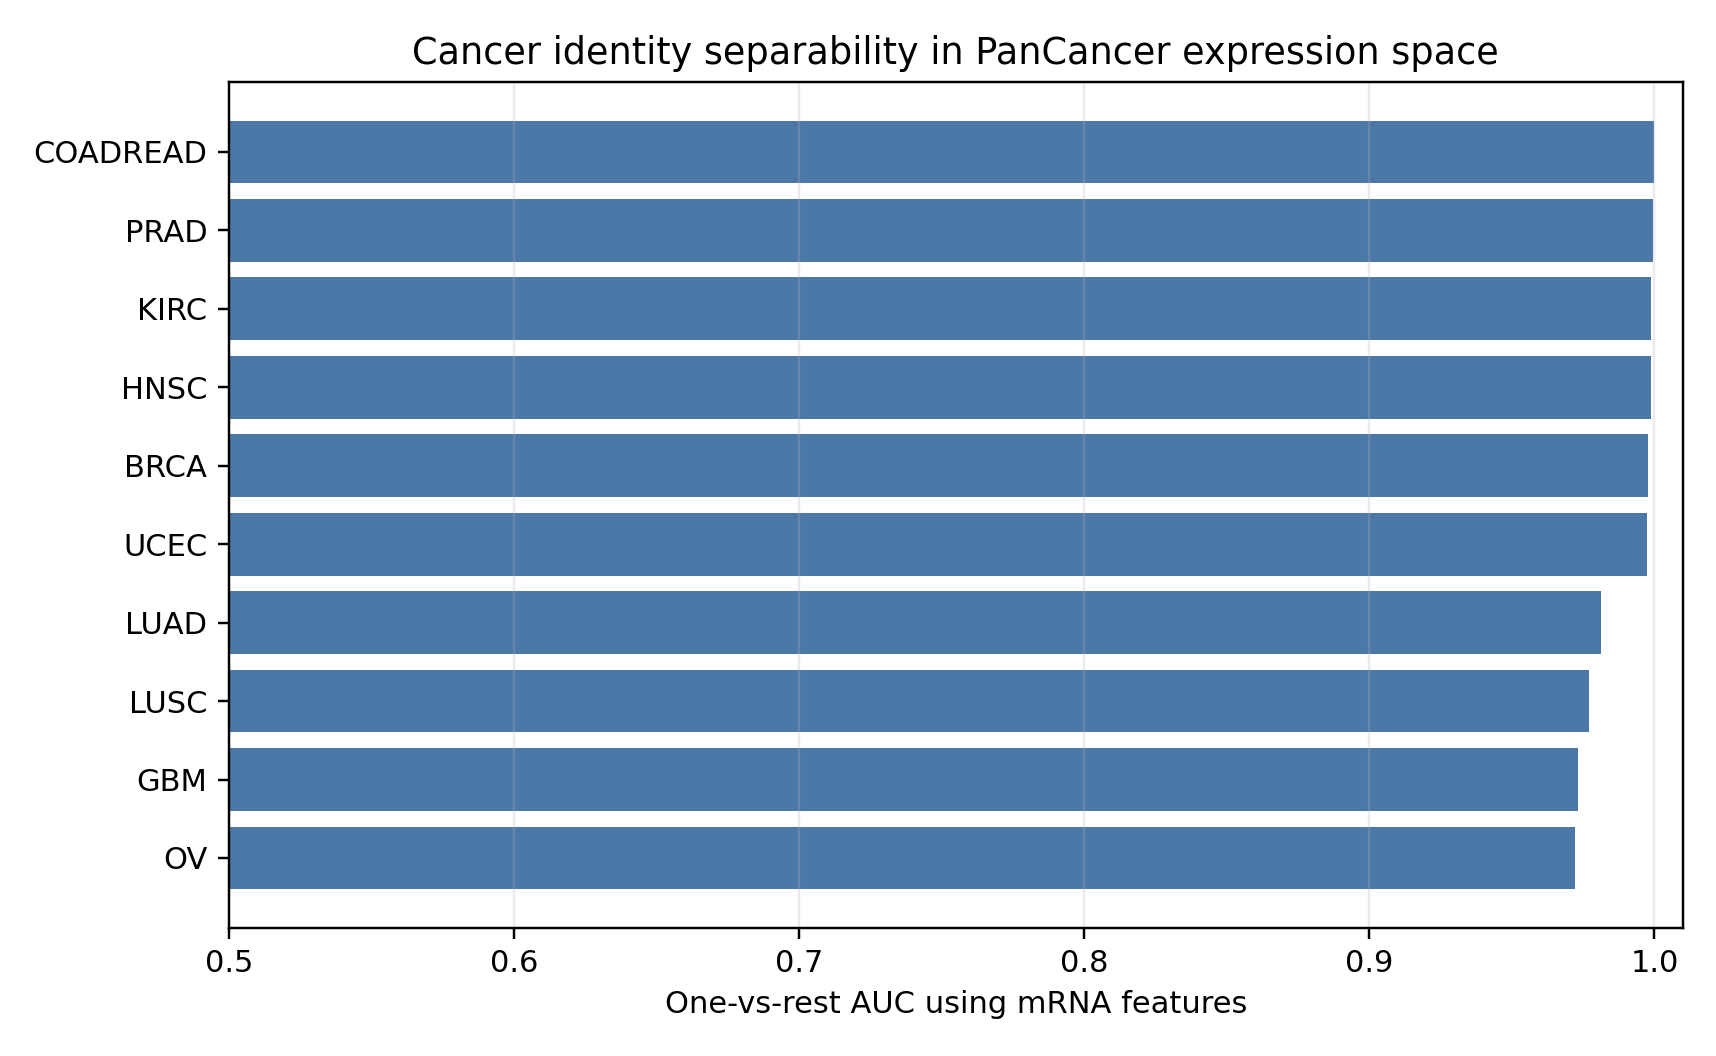
\includegraphics[width=0.86\textwidth]{figures/pancancer_cancer_separability_auc.png}
\caption{One-vs-rest cancer identity separability using mRNA features in the 10-cancer PanCancer table. All cancer types were highly separable from the rest, illustrating the strength of tissue/cancer identity signals in pan-cancer molecular data.}
\label{fig:cancer_sep}
\end{figure}

\begin{figure}[ht]
\centering
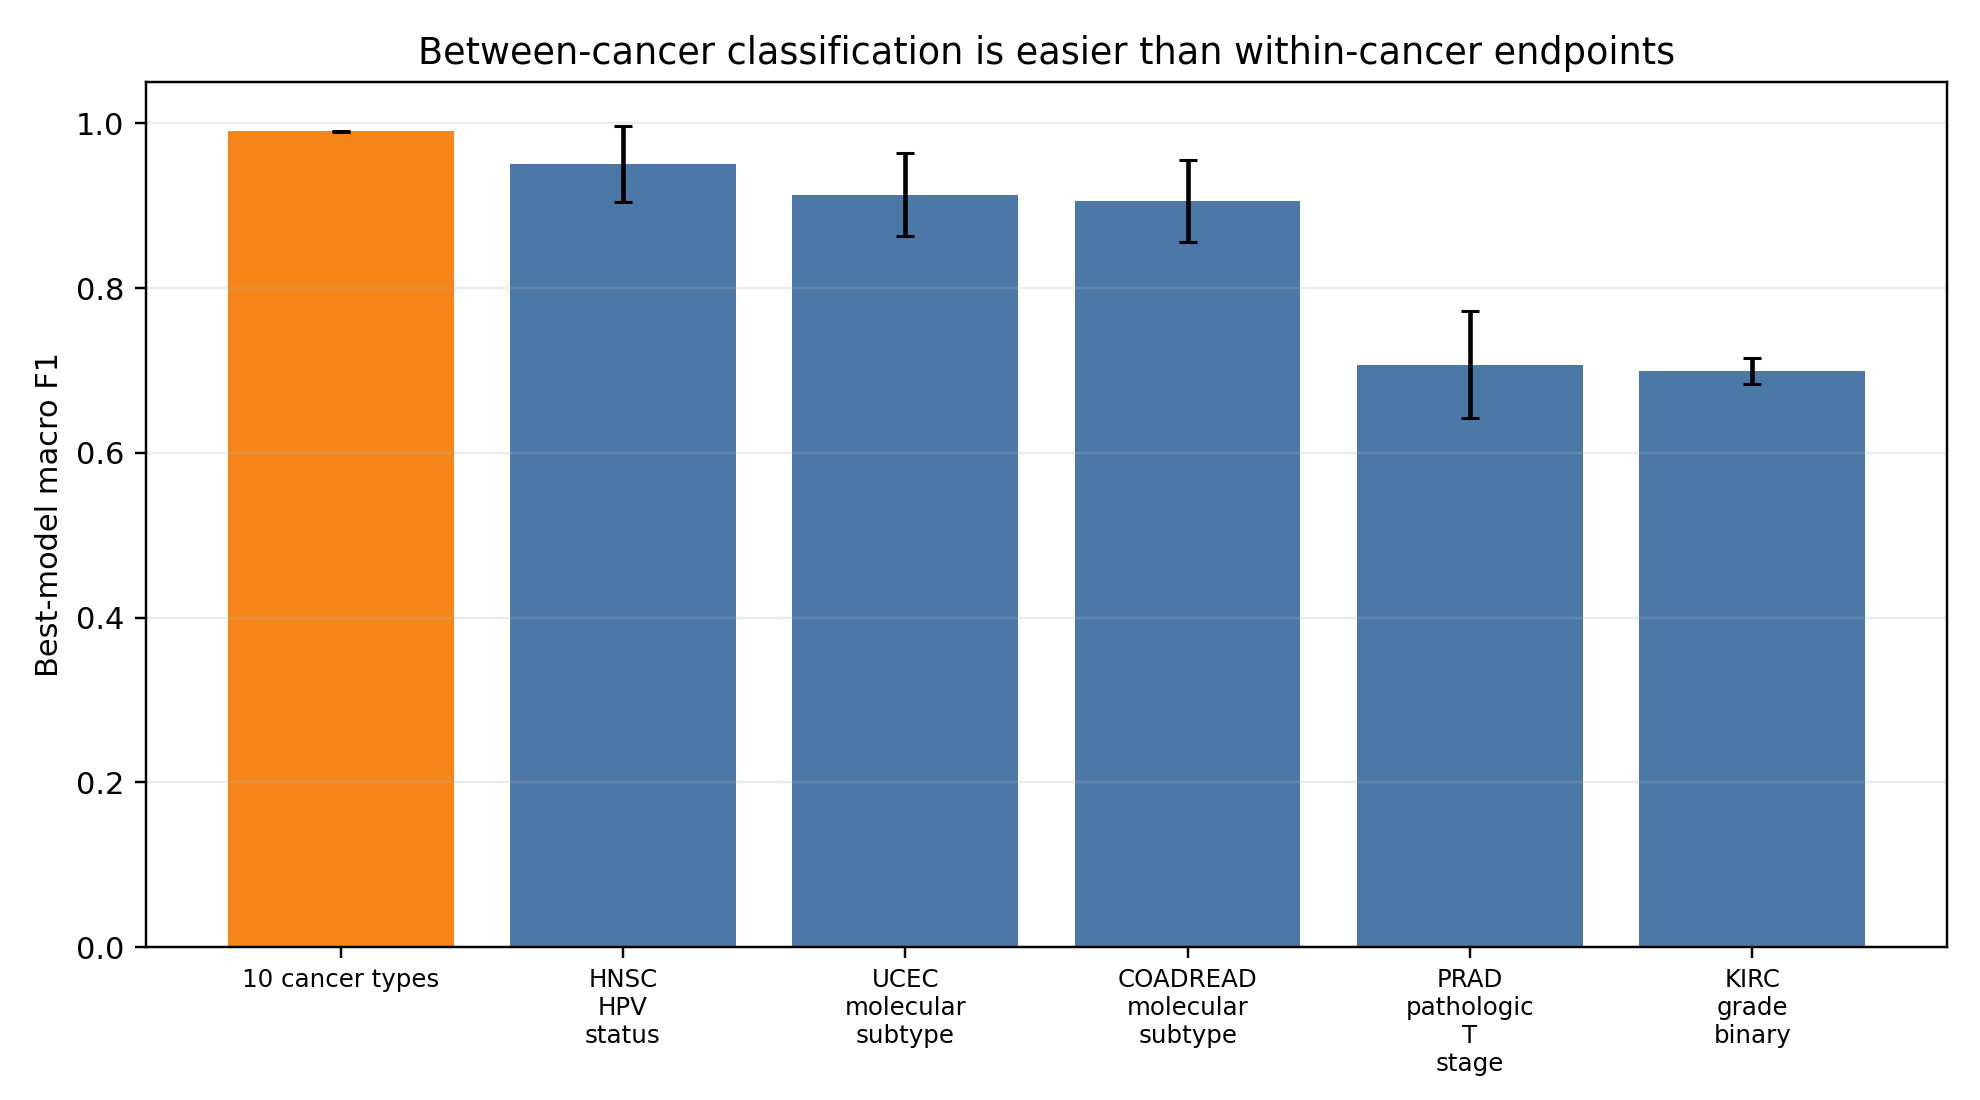
\includegraphics[width=\textwidth]{figures/pancancer_vs_internal_task_f1.png}
\caption{Best macro F1 for the 10-class PanCancer cancer-type task compared with five within-cancer endpoint tasks. The between-cancer task was substantially easier than the KIRC grade and PRAD pathologic T-stage tasks.}
\label{fig:task_difficulty}
\end{figure}

\subsection{The BRCA external-validation case study shows different shift profiles}

In the BRCA marker-expression case study, CPTAC 2020 was more separable from the TCGA/METABRIC source distribution than SMC 2018 or SCAN-B/GSE96058, with a domain separability AUC of 0.7596. SMC 2018 and SCAN-B/GSE96058 were close to random separability in this marker space (0.5165 and 0.5133, respectively). External macro F1 did not follow a simple monotonic relationship with separability: ExtraTrees performed best on SMC 2018, whereas logistic regression performed best on CPTAC 2020. These results suggest that cohort shift is not a single scalar obstacle; its effect depends on the model, label distribution, and external cohort structure.

\begin{figure}[ht]
\centering
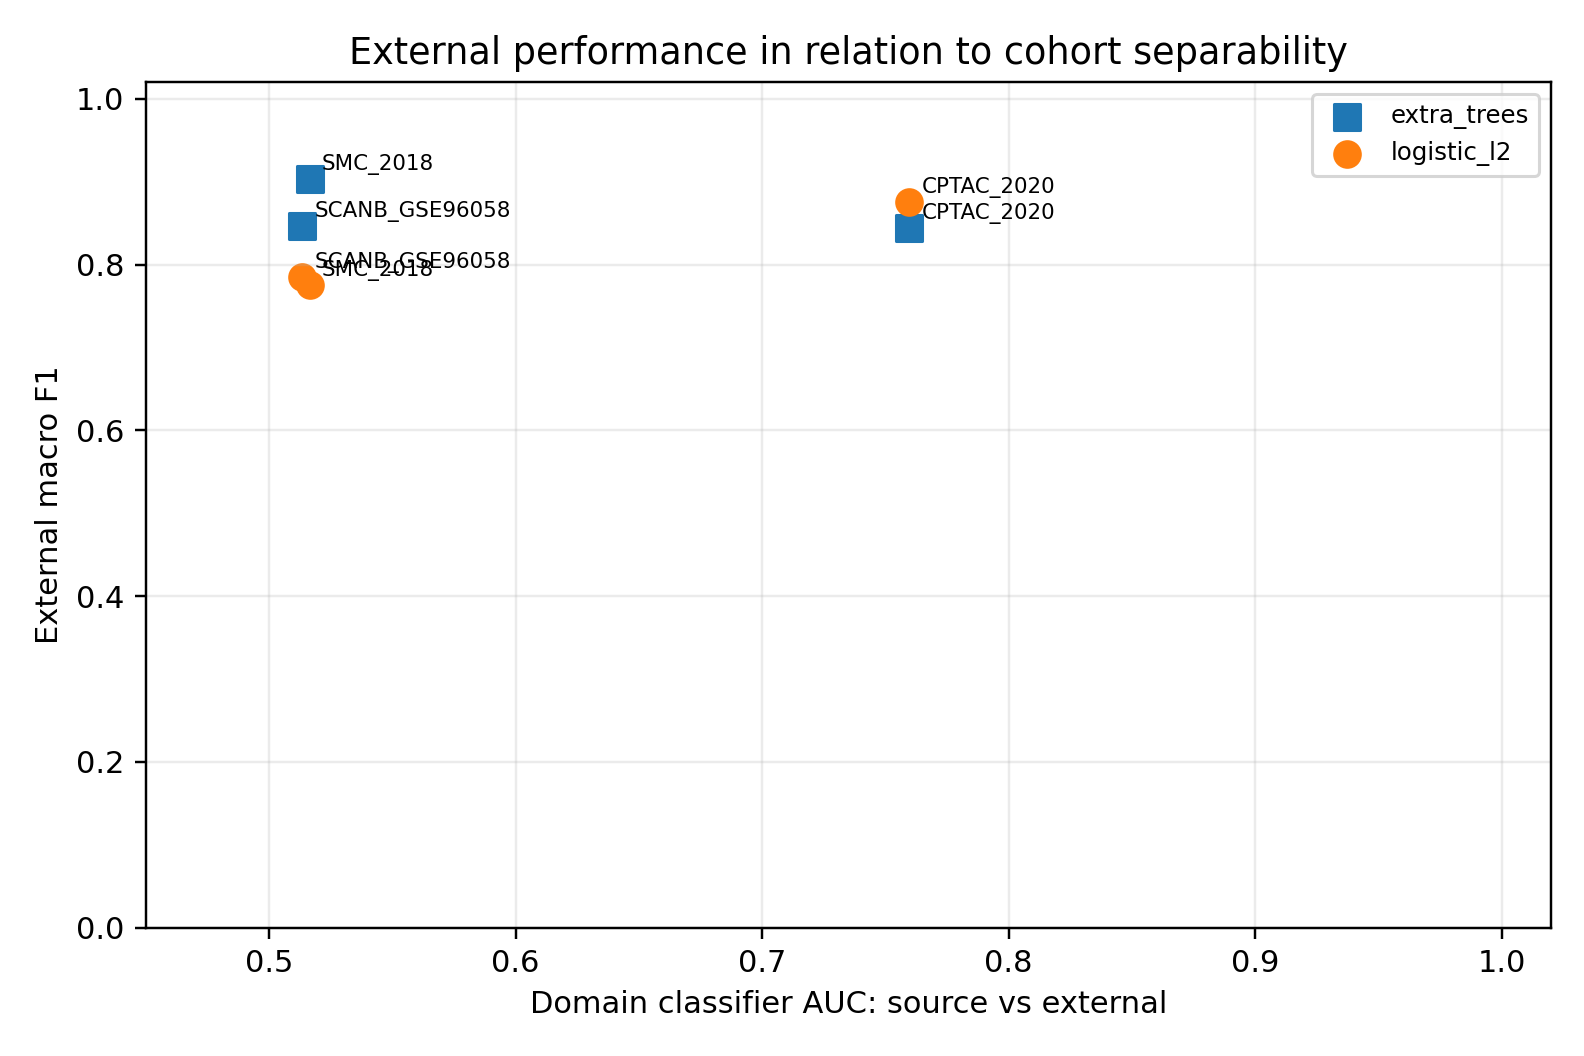
\includegraphics[width=0.86\textwidth]{figures/domain_shift_scatter.png}
\caption{BRCA external macro F1 in relation to source-versus-external cohort separability. The domain classifier AUC was computed in the 83-gene breast cancer marker expression space and transformed to separability AUC \(\max(AUC,1-AUC)\).}
\label{fig:domain_shift}
\end{figure}

\begin{table}[ht]
\centering
\caption{BRCA external-validation case study and domain-shift summary.}
\resizebox{\textwidth}{!}{%
\begin{tabular}{llrrrr}
\toprule
Dataset & Model & Macro F1 & Balanced accuracy & Mean standardized shift & Domain separability AUC \\
\midrule
CPTAC 2020 & ExtraTrees & 0.8440 & 0.8203 & 0.0384 & 0.7596 \\
SCAN-B/GSE96058 & ExtraTrees & 0.8465 & 0.8526 & 0.0381 & 0.5133 \\
SMC 2018 & ExtraTrees & 0.9028 & 0.9190 & 0.0652 & 0.5165 \\
TCGA/METABRIC validation & ExtraTrees & 0.8225 & 0.8016 & 0.0000 & 0.5000 \\
CPTAC 2020 & Logistic L2 & 0.8749 & 0.9013 & 0.0384 & 0.7596 \\
SCAN-B/GSE96058 & Logistic L2 & 0.7851 & 0.8603 & 0.0381 & 0.5133 \\
SMC 2018 & Logistic L2 & 0.7751 & 0.8732 & 0.0652 & 0.5165 \\
TCGA/METABRIC validation & Logistic L2 & 0.8219 & 0.8521 & 0.0000 & 0.5000 \\
\bottomrule
\end{tabular}
}
\label{tab:domain_shift}
\end{table}

\section{Discussion}

This study supports a data-centric view of cancer multi-omics prediction. In the five TCGA cancer-internal tasks, the same nominal multi-omics feature table behaved differently depending on modality coverage and sample pairing. The sample-level audit confirmed that the starting tables were uniquely keyed by labelled tumor sample, with no duplicate sample identifiers and high core-modality completeness. This is important because the subsequent mismatch results can be interpreted as a stress test of broken sample pairing rather than a correction for obvious duplicate rows. RPPA remained sparse at the feature level and should not be treated as a routine early-fusion modality in these tasks. More importantly, simulated sample mismatch degraded performance even though each modality's marginal distribution remained intact. This is exactly the kind of failure that can be invisible to feature-level summary statistics and visible only after sample-level alignment is audited.

The mismatch stress test also shows why a single model score can be misleading. UCEC and COADREAD were strongly affected by non-mRNA modality mismatch, especially for ExtraTrees and the Liquid-family models, whereas KIRC and PRAD were less sensitive. This does not mean that alignment is unimportant for KIRC or PRAD; rather, it means that these particular endpoints and feature sets were less dependent on cross-modal relationships under the tested models. A useful multi-omics benchmark should therefore report both performance and alignment sensitivity for classical and neural model families.

The BRCA external-validation case study adds a complementary perspective. CPTAC 2020 was more separable from the TCGA/METABRIC source distribution than SMC 2018 or SCAN-B/GSE96058 in marker expression space, yet external macro F1 depended on the model and cohort. This finding cautions against interpreting domain shift as a single scalar quantity. Domain classifier separability, standardized mean shift, class balance, label definitions, and assay compatibility should be considered together.

The 10-cancer exploratory extension clarifies a common pitfall in multi-cancer machine learning. Pan-cancer cancer-type prediction can look nearly solved, but that success mostly reflects strong tissue or cancer identity signals. It does not imply that clinically meaningful within-cancer endpoints are equally easy. The endpoint screen identified 21 candidate within-cancer tasks, but their apparent difficulty varied sharply by endpoint family: subtype tasks were generally learnable, grade tasks were cancer-dependent, and stage or T-stage tasks were often weak molecular prediction targets. Therefore, multi-cancer benchmarks should include within-cancer endpoints and should not rely only on cancer-type classification as evidence of biomedical predictive utility.

The expanded 10-fold baseline benchmark further argues against overinterpreting small model-rank differences. Although tree ensembles, logistic regression, and neural architectures each performed well in different tasks, no model family was consistently dominant across all endpoints. This is particularly relevant for Liquid/CfC-style models: their inclusion is useful as a modern neural comparator, but the present data do not justify an architecture-superiority claim. Instead, the results suggest an applicability boundary. Liquid/CfC was competitive for COADREAD, UCEC, and PRAD, but was weaker for HNSC HPV status and KIRC grade. This pattern is biologically and statistically plausible: when a simpler, high-signal decision boundary exists, regularized linear models or tree ensembles can be sufficient; when cross-modality relationships are more complex, Liquid/CfC-style modality-sequence models may be competitive. The medical interpretation table strengthens this view by linking model behavior to endpoint biology rather than treating all tasks as interchangeable labels. The stronger conclusion is methodological: benchmark studies should make sample alignment, modality coverage, endpoint biology, cohort shift, and robustness checks part of the evaluation protocol.

The main limitation is that the mismatch experiment is simulated. Real sample misalignment can arise through more complex mechanisms, including patient/sample ID mismatches, aliquot-level differences, assay-specific filtering, clinical label harmonization errors, and differences between sample, portion, analyte, and aliquot provenance. Our audit was conducted at the harmonized cBioPortal sample-identifier level; it verifies one labelled modelling row per tumor sample in the analysed tables, but it is not equivalent to a complete aliquot-level molecular provenance audit. The simulation is therefore best interpreted as a stress test of sensitivity, not as an estimate of the frequency of real errors. A second limitation is that external validation was performed as a BRCA case study. Extending the domain-shift component to external cohorts for UCEC, COADREAD, HNSC, KIRC, and PRAD would further strengthen the benchmark. A third limitation is that the 21-task endpoint screen used lightweight baselines and three-fold cross-validation for scope discovery; because endpoint discovery and apparent difficulty estimation used the same public resource, these results are subject to selection bias. Future work should apply the full 10-fold baseline, mismatch, and external-validation protocol to the most clinically important tasks identified by this screen.

Despite these limitations, the second manuscript is distinct from a model-comparison paper. Its central claim is not that one architecture is best, but that data reliability checks should be part of the benchmark itself. We recommend that cancer multi-omics prediction studies report: the sample alignment key, duplicate sample checks, modality coverage by labelled sample, coverage differences by cancer type, compatible external-cohort modality sets, training-only preprocessing, one-vs-rest domain or cancer-identity separability, and mismatch or permutation stress tests.

\section*{Data availability}

All source datasets used in this study are publicly available. TCGA PanCancer Atlas and TCGA-BRCA molecular and clinical data were accessed through cBioPortal. METABRIC, CPTAC 2020, and SMC 2018 molecular and clinical data were accessed through cBioPortal where available. GSE96058/SCAN-B data were accessed through the Gene Expression Omnibus and the associated public processed data package. Public datasets and metadata were accessed and processed through 14 July 2026. Analysis scripts, processed result tables, generated figures, reports, environment information, and manuscript source files are available in the public GitHub repository: \url{https://github.com/123hzq321/cancer-multiomics-alignment-domain-shift-benchmark}.

\section*{Code availability}

The public GitHub repository contains processed result tables required to reproduce manuscript tables and figures, along with Python scripts and package-version information. The main scripts include:
\begingroup
\footnotesize
\begin{itemize}
\item \path{scripts/analyze_alignment_domain_shift_benchmark.py}
\item \path{scripts/reviewer_cv_noise_significance_analysis.py}
\item \path{scripts/strengthen_alignment_liquid_medical_evidence.py}
\item \path{scripts/analyze_multicancer_reliability_extension.py}
\item \path{scripts/expand_multicancer_clinical_scope.py}
\end{itemize}
\endgroup

\section*{Author contributions}

Z.H. conceived the study, designed the computational experiments, processed the data, implemented the analysis pipeline, performed model training and evaluation, prepared figures and tables, and drafted the manuscript. X.B. supervised the study, contributed clinical interpretation, and revised the manuscript. Both authors reviewed and approved the final manuscript.

\section*{Competing interests}

The authors declare that they have no competing interests.

\section*{Funding}

No specific funding was received for this work.

\section*{Use of generative artificial intelligence}

Generative artificial intelligence tools were used to assist with manuscript drafting, language editing, code organization, and internal consistency checks. All analyses, interpretations, and manuscript content were reviewed and approved by the authors, who take full responsibility for the final work. No generative artificial intelligence tool is listed as an author.


\bibliographystyle{unsrt}
\bibliography{references}

\end{document}
